\hypertarget{ux57faux4e8eux4e0aux4e0bux6587ux7684ux6301ux7eedux5b66ux4e60}{%
\chapter{基于上下文的持续学习}\label{ux57faux4e8eux4e0aux4e0bux6587ux7684ux6301ux7eedux5b66ux4e60}}

\hypertarget{ux6ce8ux610fux529bux673aux5236ux4e0eux68afux5ea6ux4e0bux964dux7684ux7b49ux4ef7ux6027}{%
\section{注意力机制与梯度下降的等价性}\label{ux6ce8ux610fux529bux673aux5236ux4e0eux68afux5ea6ux4e0bux964dux7684ux7b49ux4ef7ux6027}}

注意力模块Transformer的Attention层（包含残差流在内）整体上可以被看作是一种回归问题的梯度下降优化。

\hypertarget{ux4e00ux7ebfux6027ux6ce8ux610fux529bux7684ux8868ux8fbeux5f0f}{%
\subsection{一、线性注意力的表达式}\label{ux4e00ux7ebfux6027ux6ce8ux610fux529bux7684ux8868ux8fbeux5f0f}}

对于一组token（模型输入序列）\(\{e_1,\ldots,e_n\}\) 和 query（test）token \(e_{\mathrm{test}}\)，经过去除Softmax的注意力层（即线性注意力层，后面会探讨加上Softmax的情形）后，注意力的表达式为：

\[
\mathrm{Output}_{\mathrm{test}}=e_{\mathrm{test}}+PVK^\top q_{\mathrm{test}}
\tag{1}
\]

其中输出加上自身是因为残差连接；\(P\) 为输出投影矩阵。若我们将 \(V\) 视为 \((v_1,\ldots,v_t)\)，\(K\) 视为 \((k_1,\ldots,k_t)\)，则 \(VK^\top=\sum_i v_i k_i^\top\)，即：

\[
\mathrm{Output}_{\mathrm{test}}=e_{\mathrm{test}}+P\sum_i v_i k_i^\top q_{\mathrm{test}}
\tag{2}
\]

用类似RNN的方式表述即为：

\[
S_t=S_{t-1}+v_t k_t^\top
\]

\[
\mathrm{Output}_t=\mathrm{input}_t+PS_tq_t
\]

上式意味着，我们利用隐状态矩阵 \(S\) 构建了一个从 \(K\) 到 \(V\) 的映射，并获取在输入 \(q_t\) 时的输出，作为残差相加。忽略投影 \(P\)，这里的 \(V\) 实质上拟合的是``输出与输入之间的残差''。

\hypertarget{ux4e8cux6784ux9020ux7ebfux6027ux6a21ux578bux5e76ux8bc1ux660eux7b49ux4ef7ux6027}{%
\subsection{二、构造线性模型，并证明等价性}\label{ux4e8cux6784ux9020ux7ebfux6027ux6a21ux578bux5e76ux8bc1ux660eux7b49ux4ef7ux6027}}

假设我们正在进行 In-Context Learning（上下文学习），输入是一系列示例（演示数据）：\((x_1,y_1),(x_2,y_2),\ldots,(x_N,y_N)\)，以及一个新的查询输入 \(x_{\mathrm{test}}\)。

在 Transformer 中，每个 Token 会将输入特征和标签拼接在一起。我们定义上下文矩阵为：

\[
X=[x_1,x_2,\ldots,x_N],\qquad Y=[y_1,y_2,\ldots,y_N]
\]

\textbf{输入 Token：}假设将输入特征 \(x_i\) 和目标标签 \(y_i\) 拼接成一个列向量作为 token，即：

\[
e_i=\begin{pmatrix}x_i\\y_i\end{pmatrix}
\]

引入一个由权重矩阵 \(W\in\mathbb{R}^{N_y\times N_x}\) 参数化的参考线性模型 \(y(x)=Wx\)，以及一个包含输入样本 \(x_i\) 和标签 \(y_i\) 的训练数据集 \(D=\{(x_i,y_i)\}_{i=1}^{N}\)。学习的目标是最小化平方误差损失：

\[
L(W)=\frac{1}{2N}\sum_{i=1}^{N}\|Wx_i-y_i\|^2
\]

此时梯度下降的表达式（动态模型的更新方式）为：

\[
\Delta W=-\eta\nabla_W L(W)=-\frac{\eta}{N}\sum_{i=1}^{N}(Wx_i-y_i)x_i^\top
\]

（3）

这里的 \(Wx_i-y_i\) 和前面的 \(v_i\) 对应（而不是 \(y_i\) 和 \(v_i\) 对应），表示``按原始权重的输出（\(W_0x_i\)）和应输出的值（标签 \(y_i\)）的差距''；\(x_i\) 和前面的 \(k_i\) 对应；\(\eta/N\) 和前面的 \(P\) 对应。这也就意味着，每次输入一批样本，\(W\) 的权重就将变化 \(-P\sum_i v_i k_i^\top\)。

也就是说，这个权重矩阵 \(W\) 和前面讲的隐状态矩阵 \(S\) 不一样：\(W\) 是隐式的，表示 \(x\) 到最终 \(y\) 的映射；\(S\) 是显式的，表示 \(k\) 到 \(v\)（残差 \(Wx-y\)）的映射。\(\Delta W\) 和 \(S\) 成比例关系，\(W\) 的一次梯度下降相当于运用了 \(S\) 中存储的所有上下文token的梯度。\((W+\Delta W)x_{\mathrm{test}}\) 和 \(\mathrm{input}_t+S_tq_t\) 相对应。

对于测试token：

\[
e_{\mathrm{test}}=\begin{pmatrix}x_{\mathrm{test}}\\y_{\mathrm{init}}\end{pmatrix}
\]

我们初始化 \(y_{\mathrm{init}}\) 为 \(-W_0x_{\mathrm{test}}\)（后面会阐释为什么可以这么做）。通过构造 \(W_Q\)、\(W_K\)、\(W_V\) 矩阵，使得：

当前查询 token \(j\) 的 Query 向量：

\[
q_j=W_Q e_j=\begin{pmatrix}I_x&0\\0&0\end{pmatrix}\begin{pmatrix}x_j\\y_j\end{pmatrix}=\begin{pmatrix}x_j\\0\end{pmatrix}
\]

上下文 token \(i\) 的 Key 向量：

\[
k_i=W_K e_i=\begin{pmatrix}I_x&0\\0&0\end{pmatrix}\begin{pmatrix}x_i\\y_i\end{pmatrix}=\begin{pmatrix}x_i\\0\end{pmatrix}
\]

上下文 token \(i\) 的 Value 向量：

\[
v_i=W_V e_i=\begin{pmatrix}0&0\\W_0&-I_y\end{pmatrix}\begin{pmatrix}x_i\\y_i\end{pmatrix}=\begin{pmatrix}0\\W_0x_i-y_i\end{pmatrix}
\]

计算注意力：

\[
k_i^\top q_j=(x_i^\top,0)\begin{pmatrix}x_j\\0\end{pmatrix}=x_i^\top x_j
\]

\[
\sum_{i=1}^{N}v_i(k_i^\top q_j)=\sum_{i=1}^{N}\begin{pmatrix}0\\W_0x_i-y_i\end{pmatrix}(x_i^\top x_j)
\]

\[
PVK^\top q_j=\begin{pmatrix}\eta/N&0\end{pmatrix}\left(\sum_{i=1}^{N}(W_0x_i-y_i)x_i^\top x_j\right)
\]

这意味着对上下文中的 \(W_0x-y\) 进行``聚合''，可以视为得到的是 \(W_0x_{\mathrm{test}}-y_{\mathrm{test}}\)。我们想要的就是这个上下文聚合后得到的 \(y\) 值预测 \(y_{\mathrm{test}}=(W_0+\Delta W)x_{\mathrm{test}}\)，从而上式的下面部分就可以视为 \(W_0x_{\mathrm{test}}-y_{\mathrm{test}}=-\Delta W x_{\mathrm{test}}\)，也就是``原有输出-应然输出''。而这恰好和前面 \(\Delta W\) 的表达式对上了，因此：

\[
PVK^\top q_j=\begin{pmatrix}0\\-\Delta W x_j\end{pmatrix}
\]

这意味着对于test token，（1）式等价于：

这条式子的下面部分取相反数后，也就得到参数变换后（按 \(W_0+\Delta W\)）应该输出的值，即注意力模块的输出。

\hypertarget{ux4e09ux4e3aux4ec0ux4e484ux5f0fux6709ux8d1fux53f7ux660eux660e-y_mathrmtestwx_mathrmtestdelta-wx_mathrmtestux4e3aux4ec0ux4e48ux8fd9ux91ccux662fux51cfux53bb-delta-wx_mathrmtest}{%
\subsection{\texorpdfstring{三、为什么（4）式有负号，明明 \(y_{\mathrm{test}}=Wx_{\mathrm{test}}+\Delta Wx_{\mathrm{test}}\)，为什么这里是减去 \(\Delta Wx_{\mathrm{test}}\)？}{三、为什么（4）式有负号，明明 y\_\{\textbackslash mathrm\{test\}\}=Wx\_\{\textbackslash mathrm\{test\}\}+\textbackslash Delta Wx\_\{\textbackslash mathrm\{test\}\}，为什么这里是减去 \textbackslash Delta Wx\_\{\textbackslash mathrm\{test\}\}？}}\label{ux4e09ux4e3aux4ec0ux4e484ux5f0fux6709ux8d1fux53f7ux660eux660e-y_mathrmtestwx_mathrmtestdelta-wx_mathrmtestux4e3aux4ec0ux4e48ux8fd9ux91ccux662fux51cfux53bb-delta-wx_mathrmtest}}

这需要从多轮优化的角度分析。大模型中往往是多个注意力层串行处理数据，每一轮都把输入 \(x_{\mathrm{test}}\) 转变为输出 \(y_{\mathrm{test}}\)，它又作为新的 \(x_{\mathrm{test}}\) 输入下一个注意力层。这等价于对一个线性层进行多轮权重更新：刚开始输入 \(x_{\mathrm{test}}\) 时（权重 \(W_0\)）执行一次梯度下降（权重变为 \(W_0+\Delta W\)）并输出 \(y_{\mathrm{test}}\)，它又作为新的 \(x_{\mathrm{test}}\) 输入（其他 \(x_i\) 和 \(y_i\) 仍然取原来的值）此时权重已经变为 \(W_0+\Delta W\) 的模型，再结合上下文进行梯度下降、推理，以此类推。

以上模型确实是正确的等价，但我们知道，实际上Transformer的权重是不变的，因此我们试图将上述过程再做一个等价转换，让 \(W\) 不变，而上下文 \(y_i\) 可变，更符合Transformer本身静态结构对应的表达式（即（1）式）。除了计算输出值（这一点我们已经有办法了）外，``当下的 \(W\) 值''唯一的``用处''就是用于梯度下降，而由（3）式可知，线性层梯度下降的幅度和残差 \(Wx_i-y_i\) 成正比，因此 \(W\) 从 \(W_0\) 变为 \(W_0+\Delta W\)，等价于上下文token的标签 \(y_i\) 减少 \(\Delta Wx_i\)，这时Loss不变，残差不变，优化状态不变。因此，我们可以假设多个线性层串行组成模型，每个线性层的参数均为 \(W\)，改变上下文token的 \(y_i\)：

\[
y_i^{new}=y_i-\Delta W x_i
\]

下一层的 \(W\) 不改变，但是这时候上下文token里输入的不是原始的 \(y_i\)，而是 \(y_i^{new}\)，下一层再对 \(y_i^{new}\) 进行类似的处理，以此类推，就可以通过改变上下文来等价地实现改变权重。

但是这时候会出现一个问题：自注意力层不会区分上下文token和test token，我们为了保证残差不变，把 \(y_i\) 减去 \(\Delta Wx_i\)，但是 \(y_{\mathrm{test}}=W_0x_{\mathrm{test}}+\Delta Wx_{\mathrm{test}}\)，符号反了。于是我们把 \(y_{\mathrm{init}}\) 取为 \(-W_0x_{\mathrm{test}}\)，减去 \(\Delta Wx_{\mathrm{test}}\) 后恰好为 \(-W_0x_{\mathrm{test}}-\Delta Wx_{\mathrm{test}}\)，乘以一个对角线全 \(-1\) 的输出投影矩阵即可。

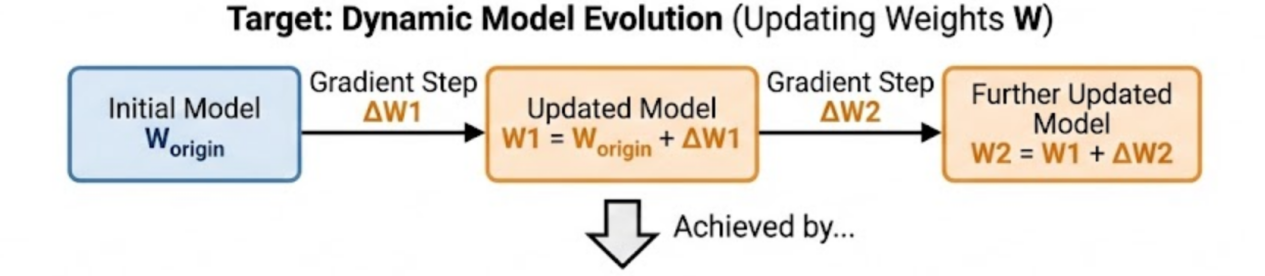
\includegraphics{images/image-0043.png}
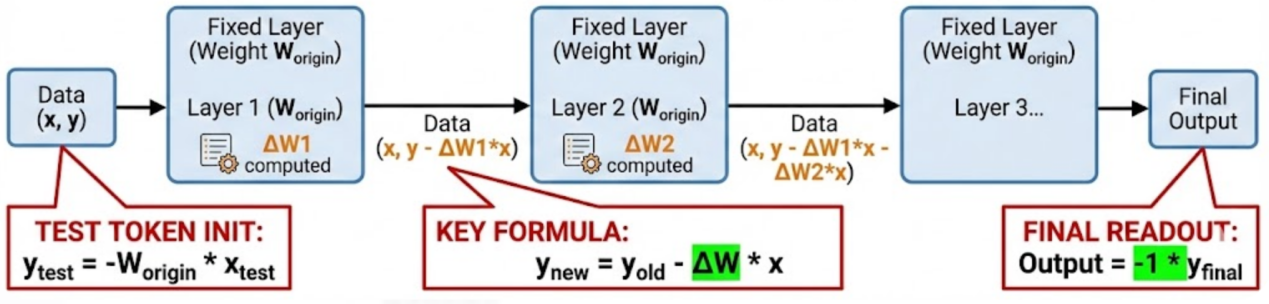
\includegraphics{images/image-0044.png}
- 穿过第 1 层注意力层（执行第 1 步梯度下降）：第 1 层根据当前的上下文计算出梯度增量 \(\Delta W_1\)。残差连接将其加上：

\[
y_{1,test}=y_{0,test}-\Delta W_1x_{\mathrm{test}}=-(W_0+\Delta W_1)x_{\mathrm{test}}
\]

\begin{itemize}
\tightlist
\item
  穿过第 2 层注意力层（执行第 2 步梯度下降）：第 2 层读取到 \(y_{1,test}\)，继续计算出新的梯度增量 \(\Delta W_2\)。残差连接再次将其加上：
\end{itemize}

\[
y_{2,test}=y_{1,test}-\Delta W_2x_{\mathrm{test}}=-(W_0+\Delta W_1+\Delta W_2)x_{\mathrm{test}}
\]

\begin{itemize}
\tightlist
\item
  穿过第 \(K\) 层注意力层（执行第 \(K\) 步梯度下降）：以此类推，经过 \(K\) 层后，测试 Token 的 \(y\) 值变成了：
\end{itemize}

\[
y_{K,test}=-W_0x_{\mathrm{test}}-\sum_{k=1}^{K}\Delta W_k x_{\mathrm{test}}
\]

\[
\hat{y}_{\mathrm{final}}=-y_{K,test}=W_0x_{\mathrm{test}}+\sum_{k=1}^{K}\Delta W_k x_{\mathrm{test}}
\]

这样，我们就把一个持续梯度下降的线性模型等价转化为了多个权重不变的线性层，数据在层间单向流动，每流过一个层，所有token（包括上下文token和test token）对应的 \(y\) 值都会减去 \(\Delta Wx\)，每一个这样的层就和Transformer中的每一个注意力层一一对应。值得注意的是，这样的 \(W_0\) 并非显式储存于Transformer的权重中，而是被隐式维护（虽然它也是不变的）：在前面的推理中，我们构造过：

\[
W_V=\begin{pmatrix}0&0\\W_0&-I_y\end{pmatrix}
\]

也就是说这里它由 \(W_V\) 决定。

总结：标准Transformer 无法在内部凭空变出一个真正的权重矩阵W存起来，只能靠修改数据流（残差）来``模拟''梯度下降，为了在多层Transformer中保证优化状态一致性，才采用了这种``别扭''的方式。

\hypertarget{ux56dbux5927ux6a21ux578bux4e2dux7684ux5b9eux9645ux60c5ux51b5}{%
\subsection{四、大模型中的实际情况}\label{ux56dbux5927ux6a21ux578bux4e2dux7684ux5b9eux9645ux60c5ux51b5}}

\hypertarget{ux4e00ux642cux8fd0ux673aux5236ux548cux5f52ux7eb3ux5934}{%
\subsubsection{（一）``搬运''机制和归纳头}\label{ux4e00ux642cux8fd0ux673aux5236ux548cux5f52ux7eb3ux5934}}

前面，我们只是在理论上证明了``自注意力有能力做梯度下降''。我们假设每个上下文token都由输入特征和标签拼接而成，但显然现实世界中的文本往往不符合这一点，输入特征和标签一般会分布在不同token中以随机位置出现。当面对这种真实随机的序列时，Transformer的第一层（包括了Softmax）并没有直接去算梯度，而是学习到了一种数据预处理功能：对于每一个含有y的token，通过q和K的匹配分数，找到它对应的x所在的token（不一定在x旁边，也不一定只有一个token），把x``搬运''到y所在的token里，再经过后面的线性层``整理''把向量变成类似于前述命题所需的(xi,yi)拼接状态。

这个搬运机制，恰好与Anthropic 团队之前发现的、被认为对上下文学习至关重要的``归纳头''（Induction Heads）现象吻合。第一层做的是Induction Head的拷贝工作，为后面开始执行真正的梯度下降（也就是前面推导的逻辑）、学习上下文铺平道路。在这里，Softmax起到了至关重要的作用：``搬运''意味着当前位置的Token必须能够百分之百地把注意力集中在目标Token（有需要的对应x值）上，同时绝对无视序列中的其他所有Token，这只有``赢家通吃''的Softmax能做到，如果纯粹用线性，往往会把序列里所有Token的特征都搅拌在一起（糊成一团），无法通过排除其他token的干扰来提取出极其干净的、单一的x。

\hypertarget{ux4e8cy_mathrminit-ux53d6ux4e3a--w_0x_mathrmtest-ux7684ux5408ux7406ux6027}{%
\subsubsection{\texorpdfstring{（二）\(y_{\mathrm{init}}\) 取为 \(-W_0x_{\mathrm{test}}\) 的合理性}{（二）y\_\{\textbackslash mathrm\{init\}\} 取为 -W\_0x\_\{\textbackslash mathrm\{test\}\} 的合理性}}\label{ux4e8cy_mathrminit-ux53d6ux4e3a--w_0x_mathrmtest-ux7684ux5408ux7406ux6027}}

而那个把 \(y_{\mathrm{init}}\) 取为 \(-W_0x_{\mathrm{test}}\) 的构造操作，在实际训练Transformer的时候，实际上只要我们将注意力权重初始化为一个非常小的值，就可以近似认为 \(W_V=0\)，进而由前面的分析 \(W_0=0\)，\(-W_0x_{\mathrm{test}}=0\)，而真实模型的第一层（归纳头）也会学习到主动把 \(y_{\mathrm{init}}\) 变换为接近0的值，在遇到test token时初始预测值就是0，随后通过层层残差连接去累加算出的梯度。

另外值得注意的是，这种模式往往只在部分层、（多头注意力的）部分头出现，后面也会阐述原因。

\hypertarget{ux4e09ux5173ux4e8e-y_mathrminit-ux4e0dux53c2ux4e0e-delta-w-ux7684ux8ba1ux7b97}{%
\subsubsection{\texorpdfstring{（三）关于 \(y_{\mathrm{init}}\) 不参与 \(\Delta W\) 的计算}{（三）关于 y\_\{\textbackslash mathrm\{init\}\} 不参与 \textbackslash Delta W 的计算}}\label{ux4e09ux5173ux4e8e-y_mathrminit-ux4e0dux53c2ux4e0e-delta-w-ux7684ux8ba1ux7b97}}

在上下文学习中，输入序列的形式为：

\[
\mathrm{Input}=[(x_1,y_1),(x_2,y_2),\ldots,(x_N,y_N),(x_{\mathrm{test}},y_{\mathrm{init}})]
\]

我们在上下文（准确地说是test token的前文）中通过梯度下降学习一个线性回归模型，再用这个模型预测 \(x_{\mathrm{test}}\) 对应的 \(y\) 值。显然，\(y_{\mathrm{init}}\) 不应该混入训练这个线性回归模型的数据，但自注意力层仍会``一视同仁''地将其纳入 \(\Delta W\) 的计算。

一种处理方法是掩码，把注意力权重矩阵对角线上的值全部设为负无穷。这将会导致训练时注意力矩阵从``下三角矩阵''变成``空心下三角矩阵''，导致为常规``下三角矩阵''设计的高度优化的Flash Attention等算子失效。

但事实上往往无需这样操作，因为根据之前的推导：

\[
V_t = W_0 x_t - y_t
\]

由前面的分析，\(-W_0x_{\mathrm{test}}=0\)，而真实模型的第一层（归纳头）也会学习到主动把 \(y_{\mathrm{init}}\) 变换为接近0的值，也就意味着此时 \(V_{\mathrm{test}}=0\)。这样，即便注意力权重没有被强制归零，它乘以的值 \(V_{\mathrm{test}}=0\)，也不会被累加到结果中，不会影响 \(\Delta W\) 的计算。

当然，真实的大模型中，显然不可能让所有test token的Value直接设为0，丢弃test token自身的信息。大模型有极其庞大的特征维度（子空间）和复杂的多头/多层分工机制，只有一部分层、一部分头是按这里所述运行的，以实现上下文学习功能；其他层、其他头中，test token的Value仍然会参与聚合，实现该token的语义处理等其他功能。真实模型不是全局丢弃了 Test Token 的 Value，而是把``提取语义''和``计算误差梯度''分给不同的注意力头去并行处理了。

值得一提的是，模型中的Attention Sink现象可能也有着类似的机制：

Transformer 每一层的公式是：输出 = 输入 + 注意力计算结果。

在深层网络中（比如 100 层的模型），很多时候，某几层可能觉得当前的特征（输入）已经足够完美了，不需要再从上下文中补充任何额外信息。此时，最理想的情况就是什么都不做，让特征顺着残差主干道原封不动地流到下一层。也就是说，模型希望：注意力计算结果 = 0，从而实现输出 = 输入 + 0。

但是，注意力机制里有一个极其霸道的数学公式：Softmax。Softmax 要求：所有 Token 的注意力权重加起来，必须 100\% 等于 1.0。

既然被逼着必须把 100\% 的注意力分配出去，而自己又不想改变特征，大模型（比如 Llama、GPT）在漫长的预训练中，自己``顿悟''出了一个绝招：

\begin{enumerate}
\def\labelenumi{\arabic{enumi}.}
\tightlist
\item
  找一个替罪羊（Sink Token）：模型通常会选中序列的第一个 Token（比如 \texttt{\textless{}s\textgreater{}}）或者第一个标点符号。
\item
  把它的 Value 变成 0：模型在训练参数时，偷偷把提取这个替罪羊 Value 的权重矩阵学成一种特殊状态，使得这个替罪羊的 \(V_{sink} \approx 0\)。
\item
  倾泻无用的注意力：当模型在某一层``不想关注任何上下文''时，它就强行把高达 99\% 的注意力分数（Attention Score）打给这个替罪羊。
\end{enumerate}

见证奇迹的时刻到了：这 99\% 的注意力权重乘上替罪羊的 \(V_{sink}\)：

\[
0.99 \times 0 = 0
\]

于是，整个注意力分支的计算结果变成了 0。输出 = 输入 + 0。模型成功地在满足 Softmax 苛刻要求的同时，完美地什么也没做，保持了特征的纯洁。

\hypertarget{ux56dbux771fux5b9eux8fd0ux884cux4e2dux54eaux4e9btokenux7684vux4f1aux88abux7f6eux4e3aux96f6}{%
\subsubsection{（四）真实运行中，哪些token的V会被置为零？}\label{ux56dbux771fux5b9eux8fd0ux884cux4e2dux54eaux4e9btokenux7684vux4f1aux88abux7f6eux4e3aux96f6}}

在真实的自回归序列中，输入不是拼好的 \((x,y)\)，而是每个 \(x\) 和 \(y\) 都分布在不同 token 中，如一个交替序列：\(x_1,y_1,x_2,y_2,\ldots,x_{19},y_{19},x_{20}\)。

当我们要生成 \(y_{19}\) 时（这时 \(y_{19}\) 还没有产生，被初始化为 \(0\)；test token 为 \(x_{19}\)）：

\begin{itemize}
\tightlist
\item
  浅层网络处理：因为这是新输入的 token，它还没有对应的 \(y_{19}\)。它的隐藏层状态只能是 \((x_{19},0)\)。
\item
  深层网络（梯度下降层）：深层网络提取它的 Value 向量。根据公式 \(V = W_0x - y\)，此时 \(V_{19}=W_0x_{19}-0 \approx 0\)。
\item
  结果：它完美地扮演了 Test Token，带着 \(V_{19}=0\) 去和前面的 KV Cache 算注意力，输出预测结果 \(\hat{y}_{19}\)。
\item
  物理沉淀：第 19 位的 KV Cache 被永久固化，其深度层的 \(V\) 永远是 0。
\end{itemize}

此时梯度下降用的是 \((x_1,y_1),(x_2,y_2),\ldots,(x_{18},y_{18})\)。\(x_{19}\) token 的 \(V\) 于是在KV Cache中被固化为 \(0\)。

注意：这里的深层网络不是最终的输出层，只是部分隐藏层的部分头。最终输出层的Value向量并不是0，无需担心信息损失。

当我们要生成 \(x_{20}\) 时（test token 为 \(y_{19}\)）：

\begin{itemize}
\tightlist
\item
  浅层网络处理（复制机制启动）：大模型的第 1 层（通常是 Softmax 归纳头）具有强大的时序视野。当它处理处于第 20 位的 \(y_{19}\) 时，它会向回看一眼第 19 位的 \(x_{19}\)，并把 \(x_{19}\) 的特征复制到自己的隐藏层状态中。
\item
  深层网络（梯度下降层）：当数据流到深层时，第 20 位的隐藏状态已经不再是单薄的 \(y_{19}\)，而是被浅层网络组装成了完整的上下文对 \((x_{19},y_{19})\)。
\item
  根据公式，深层网络在计算第 20 位的 Value 向量时：
\end{itemize}

\[
V_{20} = W_0x_{19} - y_{19} \ne 0
\]

\begin{itemize}
\tightlist
\item
  物理沉淀：第 20 位的 KV Cache 被固化，其深度层包含了一个非零的 \(V_{20}\)。
\end{itemize}

此时梯度下降用的还是 \((x_1,y_1),(x_2,y_2),\ldots,(x_{18},y_{18})\)。（不能包括 \((x_{19},y_{19})\)，因为这是 test token）

\(V_{y_{19}}=W_0x_{19}-y_{19}\ne 0\)。这一次计算后，KV Cache包含了一个非零的 \(V_{y_{19}}\)。

当我们要生成 \(y_{20}\) 时（test token 为 \(x_{20}\)）：

\(x_{20}\) 作为Query去遍历过去的KV Cache。

此时梯度下降用的是 \((x_1,y_1),(x_2,y_2),\ldots,(x_{18},y_{18}),(x_{19},y_{19})\)。

对于 \(x_{19}\)，它的 \(V_{19}=0\)，乘法结果为 \(0\)，直接被无视；对于 \(y_{19}\)，它的 \(V_{y_{19}}=W_0x_{19}-y_{19}\ne 0\)，提供了第 19 个样本的梯度信息。

\hypertarget{ux4e94transformerux5185ux90e8ux53eaux662fux6734ux7d20ux7684ux68afux5ea6ux4e0bux964dux5417}{%
\subsubsection{（五）Transformer内部只是朴素的梯度下降吗？}\label{ux4e94transformerux5185ux90e8ux53eaux662fux6734ux7d20ux7684ux68afux5ea6ux4e0bux964dux5417}}

部分后续研究指出，给Transformer喂了条件数极差的数据（特征矩阵极度不平衡）的情况下，其性能远优于普通的梯度下降。根据对中间层输出的分析，Transformer可能在内部自动收敛成了一个类似于迭代牛顿法的收敛轨迹，从而能在极短的Few-shot样本下瞬间学会新任务。

\hypertarget{ux4e94ux542bsoftmaxux7684ux60c5ux5f62}{%
\subsection{五、含Softmax的情形}\label{ux4e94ux542bsoftmaxux7684ux60c5ux5f62}}

\hypertarget{ux4e00ux5355ux5934softmaxux7684ux56f0ux5883ux5f15ux5165ux7ebfux6027ux504fux79fb}{%
\subsubsection{（一）单头Softmax的困境：引入线性偏移}\label{ux4e00ux5355ux5934softmaxux7684ux56f0ux5883ux5f15ux5165ux7ebfux6027ux504fux79fb}}

单层、单头的Softmax自注意力层无法完全匹配普通梯度下降的性能。其根本原因在于，Softmax的指数运算和归一化分母会在矩阵乘法中产生一个附加的误差项。这可以通过一阶泰勒展开近似说明。

在自注意力机制中，Softmax 函数作用于注意力分数（即 Query 和 Key 的内积）。对于当前的查询 Token \(x_j\) 和第 \(i\) 个上下文 Token \(x_i\)，未归一化的注意力分数为：

\[
z_i = k_i^T q_j = x_i^T W_{KQ}x_j
\]

将包含所有 \(N\) 个上下文 Token 的分数代入 Softmax 函数，第 \(i\) 个位置的输出为：

\[
\mathrm{softmax}(z)_i = \frac{e^{z_i}}{\sum_{k=1}^{N} e^{z_k}}
\]

根据高等数学中的一阶泰勒展开公式，当 \(z \to 0\) 时，指数函数可以近似为：

\[
e^z \approx 1 + z
\]

将这个近似代入 Softmax 的分子和分母中：

\begin{itemize}
\tightlist
\item
  分子：
\end{itemize}

\[
e^{x_i^T W_{KQ}x_j} \approx 1 + x_i^T W_{KQ}x_j
\]

\begin{itemize}
\tightlist
\item
  分母：
\end{itemize}

\[
\sum_{k=1}^{N} e^{x_k^T W_{KQ}x_j} \approx \sum_{k=1}^{N}(1+x_k^T W_{KQ}x_j)
\]

将所有 \(N\) 个 Token 的分子写成一个列向量：

\[
\begin{pmatrix}
1+x_1^T W_{KQ}x_j \\
\vdots \\
1+x_N^T W_{KQ}x_j
\end{pmatrix}
=
\mathbf{1}+
\begin{pmatrix}
x_1^T W_{KQ}x_j \\
\vdots \\
x_N^T W_{KQ}x_j
\end{pmatrix}
= \mathbf{1}+K^Tq_j
\]

其中 \(\mathbf{1}\) 是一个全为 1 的列向量。令分母的和为标量 \(S\)。那么 Softmax 的输出向量可以写为：

\[
\mathrm{softmax}(K^Tq_j) \approx \frac{1}{S}(\mathbf{1}+K^Tq_j)
= \frac{1}{S}K^Tq_j+\frac{1}{S}\mathbf{1}
\]

因此有：

\[
\mathrm{softmax}(K^Tq_j) \propto K^Tq_j+\mathbf{1}
\]

物理含义：这个 \(\epsilon\) 是一个常数偏移量（Linear Offset）。它意味着，即使某些 Token 和当前 Query 毫无关系（内积 \(x_i^TW_{KQ}x_j=0\)），Softmax 依然会强制分配给它们一个基础的权重（即 \(\frac{1}{S}\)）。这种``强制均分''的特性，污染了原本纯净的梯度方向，导致单头 Softmax 注意力无法完美执行梯度下降。
即便对于内积为负数的token（对应可能是数学推导中的错误方向），权重也会变成正值。这显然不合理。

\hypertarget{ux4e8cux591aux5934softmaxux5982ux4f55ux89e3ux51b3ux8fd9ux4e00ux95eeux9898}{%
\subsubsection{（二）多头Softmax如何解决这一问题}\label{ux4e8cux591aux5934softmaxux5982ux4f55ux89e3ux51b3ux8fd9ux4e00ux95eeux9898}}

前面提过，由于Softmax对于归纳头起着不可或缺的作用，我们无法通过直接去掉Softmax的方法来增强上下文学习能力。但既然偏移量1（即epsilon）为常数，那么多头Softmax可以通过不同头之间相减抵消来实现：

假设模型学习到了两个注意力头，并且在最后的输出投影层（Projection Layer）中，它将这两个头的权重学成了符号相反的形式，即使得 \(P_1V_1 \approx -P_2V_2\)。为了简化表达，论文假设这两个头提取误差的矩阵 \(PV\) 相同（或被网络调整到一致），但在内部的注意力特征矩阵 \(W_{KQ}\) 上学到了不同的特征空间。

我们将这两个头的注意力计算结果相减：

\[
\mathrm{Output} \approx PV \cdot \mathrm{softmax}(K_1^Tq_{1,j}) - PV \cdot \mathrm{softmax}(K_2^Tq_{2,j})
\]

将我们在第一部分得到的泰勒近似列向量代入上式（这里论文做了一个合理假设，即两个头经过 Softmax 的分母常数 \(S\) 近似相等，并将其吸收到 \(PV\) 中）：

\[
\mathrm{Output} \approx PV \left[
\begin{pmatrix}
1+x_1^TW_{1,KQ}x_j \\
\vdots
\end{pmatrix}
-
\begin{pmatrix}
1+x_1^TW_{2,KQ}x_j \\
\vdots
\end{pmatrix}
\right]
\]

接下来进行极其简单的线性代数运算，将对应行的元素相减。对于第 \(i\) 行：

\[
\begin{aligned}
(1+x_i^TW_{1,KQ}x_j)-(1+x_i^TW_{2,KQ}x_j)
&= 1-1+x_i^TW_{1,KQ}x_j-x_i^TW_{2,KQ}x_j \\
&= x_i^T(W_{1,KQ}-W_{2,KQ})x_j
\end{aligned}
\]

看，常数项 1（即那个讨厌的 \(\epsilon\) 偏移量）在减法中完美归零了。

\hypertarget{ux516dux4e3aux4ec0ux4e48transformerux4f5cux4e3aux4e00ux79cdux4e8bux5b9eux4e0aux7684ux5143ux5b66ux4e60ux7b97ux6cd5ux4ecdux4e0dux80fdux5f88ux597dux5730ux5e94ux5bf9oodux95eeux9898}{%
\subsection{六、为什么Transformer作为一种事实上的元学习算法，仍不能很好地应对OOD问题？}\label{ux516dux4e3aux4ec0ux4e48transformerux4f5cux4e3aux4e00ux79cdux4e8bux5b9eux4e0aux7684ux5143ux5b66ux4e60ux7b97ux6cd5ux4ecdux4e0dux80fdux5f88ux597dux5730ux5e94ux5bf9oodux95eeux9898}}

\hypertarget{ux4e00ux7279ux5f81ux63d0ux53d6ux7684ux56f0ux96be}{%
\subsubsection{（一）特征提取的困难}\label{ux4e00ux7279ux5f81ux63d0ux53d6ux7684ux56f0ux96be}}

我们在前面推导中的前提是，执行梯度下降的特征向量 \(x\)，是经过大模型的Embedding和MLP层投影后的深层表示。注意力层可以看成实时梯度下降，即视为元学习；但Embedding和MLP层并不是如此。如果遇到OOD问题（比如人类从未见过的数据模态），预训练阶段的MLP根本没有为这种数据建立特征坐标系。OOD数据在输入网络后，被MLP映射成了一堆毫无意义的噪声向量，无法顺利提取数据的特征，进而后续的注意力层在执行 \(y_{new}=y_{old}-\Delta Wx\) 时，算出的梯度也就是一团乱码。

\hypertarget{ux4e8cux68afux5ea6ux4e0bux964dux7684ux5c40ux9650ux6027}{%
\subsubsection{（二）梯度下降的局限性}\label{ux4e8cux68afux5ea6ux4e0bux964dux7684ux5c40ux9650ux6027}}

梯度下降算法本身的特点决定了，面对OOD任务时，大模型所谓的``学习''，并不是真正在寻找全局最优解，而是在它预训练时见过的``任务池''里，寻找一个和当前OOD任务最相似的替代品。它只能在已有的先验知识流形（Manifold）上插值，无法外推到一个全新的物理空间。

\hypertarget{ux4e09ux8ba1ux7b97ux6df1ux5ea6ux4e0dux8db3}{%
\subsubsection{（三）计算深度不足}\label{ux4e09ux8ba1ux7b97ux6df1ux5ea6ux4e0dux8db3}}

我们证明了：1层Transformer = 1步梯度下降。一个100层的模型，最多也只能执行几十步、上百步的有效梯度下降。而真正的OOD任务（比如从头训练一个视觉模型）往往需要几万、几十万步的梯度迭代才能收敛。大模型那极其有限的层数，根本无法提供足够的计算深度来完成OOD的参数拟合。

当然，随着RLVR带来的模型推理能力的提升，模型在完成一个任务（即上下文不清空）的情况下的KV Cache更新次数和有效计算深度大大增加。``组合型OOD''往往能被解决：如给一道全新的数学竞赛题，整体来看它是OOD的，但它可以把这个问题拆解，原子步骤（加减乘除、代数变换）都在它的先验特征空间内，RL训练出的思维链能通过千万步的内部梯度下降，把这些已知特征重新组合，最终攻克难题。但对于``绝对型OOD''，即输入的底层特征在模型的MLP中根本不存在映射的情况，该方法仍然无效。

\hypertarget{ux4e03ux4f18ux5316ux95eeux9898ux7684ux7b49ux4ef7ux6027}{%
\subsection{七、优化问题的等价性}\label{ux4e03ux4f18ux5316ux95eeux9898ux7684ux7b49ux4ef7ux6027}}

在神经心理学中，记忆是由输入引起的神经更新，而学习是获取有效和有用记忆的过程。我们遵循 Behrouz 等人的定义：

\textbf{定义 1（联想记忆）}：给定一组键（Keys）\(\mathcal{K}\subseteq\mathbb{R}^{d_k}\) 和值（Values）\(\mathcal{V}\subset\mathbb{R}^{d_v}\)，联想记忆是一个算子 \(\mathcal{M}:\mathcal{K}\to\mathcal{V}\)，用于映射这两组集合。为了从数据中学习这种映射，我们定义一个目标函数 \(\tilde{\mathcal{L}}(\cdot;\cdot)\) 来衡量映射的质量，\(\mathcal{M}\) 可以定义为：

\[
\mathcal{M}^*=\arg\min_{\mathcal{M}}\tilde{\mathcal{L}}(\mathcal{M}(\mathcal{K});\mathcal{V})
\tag{1}
\]

原理阐释与推导分析：

\begin{itemize}
\tightlist
\item
  核心思想：这里将``记忆''看作是一个函数 \(\mathcal{M}\)。传统的观点认为训练模型是调整参数，而这里的观点是：训练过程本身就是在一个函数空间中寻找最优解，使得这个函数能最好地把 Key 映射到 Value。
\item
  物理意义：方程 (1) 本质上是在说，最佳的记忆状态 \(\mathcal{M}^*\) 是那个能最小化预测误差的状态。在深度学习中，\(\mathcal{K}\) 通常是输入数据，\(\mathcal{V}\) 是标签或目标，\(\tilde{\mathcal{L}}\) 是损失函数。NL 的独特之处在于，它认为模型内部的每一个组件（甚至是优化器）都在解这样一个方程。
\end{itemize}

事实上，无论是Attention注意力模块的前向计算，还是传统意义上的``优化''，都可以视为这样一个``寻找最优函数''的过程。下面我们推导梯度下降法与其的等价性：

假设我们要用梯度下降法训练一个单层 MLP（参数为 \(W\)）。优化目标是：

\[
W^*=\arg\min_W\mathcal{L}(W;\mathcal{D}_{train})
\]

梯度下降的更新规则导致权重更新等价于：

\[
W_{t+1}=W_t-\eta_{t+1}\nabla_{W_t}\mathcal{L}(W_t;x_{t+1})
\]

这里 \(x_{t+1}\) 是在 \(t+1\) 时刻输入的一个批量训练数据。由于 \(y_{t+1}=W_tx_{t+1}\)，对 \(W_t\) 的梯度即为对 \(y_{t+1}\) 的梯度和 \(x_{t+1}\) 的积：

\[
W_{t+1}=W_t-\eta_{t+1}\nabla_{y_{t+1}}\mathcal{L}(W_t;x_{t+1})\otimes x_{t+1}
\tag{4}
\]

设 \(W_t\) 为此时模型的权重，\(x_{t+1}\) 为当前的输入，\(y_{t+1}=W_tx_{t+1}\) 为模型在当前权重的线性输出。我们把损失函数 \(\mathcal{L}(W_t;x_{t+1})\) 称为``惊讶程度''。这既是因为模型预测越正确，惊讶程度越低，也是因为交叉熵损失函数的信息论背景本来就是``惊讶度''。

我们定义``惊奇信号''为：

\[
u_{t+1}\triangleq \nabla_{y_{t+1}}\mathcal{L}(W_t;x_{t+1})
\]

其中：

\begin{itemize}
\tightlist
\item
  \(W_t\)：当前时刻的模型权重。
\item
  \(x_{t+1}\)：当前的输入数据。
\item
  \(y_{t+1}=W_tx_{t+1}\)：模型在当前权重的线性输出（假设是单层 MLP）。
\item
  \(\mathcal{L}\)：损失函数。
\end{itemize}

它可以理解为``Loss对神经网络输出层的指令''，即怎样调整网络的输出y，以使损失最小。

预测误差的直接体现：\(u_{t+1}\)（即 \(\nabla_y\mathcal{L}\)）直接衡量了模型当前的输出 \(y_{t+1}\) 和真实标签（或目标）之间的差距。

对于 \(t+1\) 时刻新输入的数据 \(x_{t+1}\)，如果我们只需要根据用已有数据训练出来的 \(W_t\)，就能将输入转化为正确标签 \(y_{t+1}\)，那么权重 \(W_t\) 已经是最优了，完全没有必要更新，\(u_{t+1}=0\)。反之，如果预测和 \(y_{t+1}\) 相差很大，惊讶程度就会很高，则意味着 \(W_t\) 需要较大的调整。

举一个例子：

\begin{enumerate}
\def\labelenumi{\arabic{enumi}.}
\tightlist
\item
  输入 \(x\)：``The sky is\ldots{}''
\item
  模型预测 \(y\)：``\ldots green''（绿色）
\item
  真实标签：``\ldots blue''（蓝色）
\end{enumerate}

在这个过程中：

\begin{itemize}
\tightlist
\item
  \(\mathcal{L}\)（惊讶程度）：模型发现真实是 Blue 而不是 Green，非常震惊。Loss 值很大（比如 5.0），这就是``惊讶程度''。
\item
  \(u_{t+1}\)（惊奇信号）：这个信号是一个向量，它告诉模型具体的误差信息：``Green 的概率太高了，要降低！''``Blue 的概率太低了，要升高！''这个向量 \(u_{t+1}\) 就是具体的``修正指令''。
\item
  Nested Learning 的记忆过程：模型会把这次经历存进 MLP：``当你下次看到 `The sky is\ldots{}'（\(x\)）时，记得要把那个叫 \(u\) 的修正指令调出来。''
\end{itemize}

这可以解释为什么神经网络（如MLP）可以作为记忆模块。训练前的神经网络里没有信息，给定一个输入x，它的输出y是一个噪声（先验为噪声分布）。而``训练''的过程，就可以视为告诉神经网络：``下次再遇到x，你的输出应该往u方向移动。''或者说，就是让它``记忆''输入与``碰到这个输入时，怎么（从先验的随机状态开始）改变自己的输出''之间的关系。

或者说，MLP的梯度下降更新本质是一个``压缩''过程，将当前输入数据及其对应``怎么修改输出''的信息``压缩''进权重中。模型通过持续进行在线梯度下降（Online Gradient Descent），实时地修改自己的神经网络权重，存储读过的数据片段的信息。

更进一步地说，惊奇信号的含义实际上是一种``反思''，即``根据当前神经网络输出与目标（标签）的差距来看，我的权重应该做怎样的改进''，并将反思写入权重，让模型实现在推理阶段的持续改进。

下面我们再以优化视角看这个问题：

同式 (4)，由于 \(y_{t+1}=Wx_{t+1}\) 是模型输出，我们可以令 \(u_{t+1}=\nabla_{y_{t+1}}\mathcal{L}(W_t;x_{t+1})\)，并将反向传播过程重新表述为寻找最优联想记忆的优化问题的解。也就是说，我们旨在找到映射输入 \(x_{t+1}\) 到其对应的 \(u_{t+1}\) 的最佳 \(W\)：

\[
W_{t+1}=\arg\min_W \langle Wx_{t+1},u_{t+1}\rangle+\frac{1}{2\eta_{t+1}}\lVert W-W_t\rVert_2^2
\tag{5}
\]

\[
=\arg\min_W\left\langle Wx_{t+1},\nabla_{y_{t+1}}\mathcal{L}(W_t;x_{t+1})\right\rangle+\frac{1}{2\eta_{t+1}}\lVert W-W_t\rVert_2^2
\tag{6}
\]

这条表达式的第一项是 \(Wx_{t+1}\)（输出）和 \(u_{t+1}\)（Loss 对输出的梯度）的点积相似度，\(W\) 的更新会让输出尽量沿着梯度的反方向；第二项是正则化项，避免权重更新过大。这一步将梯度下降公式逆向推导回了一个优化问题。

定义目标函数：

\[
J(W)=\left\langle Wx_{t+1},u_{t+1}\right\rangle+\frac{1}{2\eta_{t+1}}\lVert W-W_t\rVert_2^2
\]

步骤 1：对第一项求导。利用矩阵微分性质 \(\langle A,B\rangle=\mathrm{Tr}(A^\top B)\)，可得到：

\[
\frac{\partial}{\partial W}\left\langle Wx_{t+1},u_{t+1}\right\rangle
=\frac{\partial}{\partial W}\left(u_{t+1}^{\top}Wx_{t+1}\right)
=u_{t+1}x_{t+1}^{\top}
\]

注意：这里 \(u_{t+1}x_{t+1}^{\top}\) 正是外积形式的梯度项。

步骤 2：对第二项求导：

\[
\frac{\partial}{\partial W}\left(\frac{1}{2\eta_{t+1}}\lVert W-W_t\rVert_2^2\right)
=\frac{1}{2\eta_{t+1}}\cdot 2(W-W_t)
=\frac{1}{\eta_{t+1}}(W-W_t)
\]

步骤 3：求解使梯度为零的条件：

\[
\nabla_W J(W)=u_{t+1}x_{t+1}^{\top}+\frac{1}{\eta_{t+1}}(W-W_t)=0
\]

因此：

\[
W=W_t-\eta_{t+1}(u_{t+1}x_{t+1}^{\top})
\]

带动量的梯度下降也可以类似看待：

接下来，我们引入动量项。更新规则如下：

\[
W_{t+1}=W_t-m_{t+1}
\tag{7}
\]

\[
m_{t+1}=m_t+\eta_{t+1}\nabla_{W_t}\mathcal{L}(W_t;x_{t+1})
\tag{8}
\]

这里把 \(m_{t+1}\) 定义为从 \(W_t\) 中减去的更新量，因此它沿当前梯度方向累积；真正的参数更新仍然通过 \(W_{t+1}=W_t-m_{t+1}\) 沿负梯度方向前进。在方程 8 中，如果令 \(g_{t+1}=\nabla_{W_t}\mathcal{L}(W_t;x_{t+1})\)，那么方程 8 可以被重写为：

\[
m_{t+1}=\arg\min_m-\left\langle m,g_{t+1}\right\rangle
+\frac{1}{2\eta_{t+1}}\lVert m-m_t\rVert_2^2
\tag{10}
\]

分层结构：

\begin{itemize}
\tightlist
\item
  第 1 层（外层）：更新权重 \(W\)。它使用的是 \(m\) 的值。
\item
  第 2 层（内层）：更新动量 \(m\)。方程 (10) 表明，更新动量 \(m\) 的过程，实际上是在求解一个优化问题，目的是让 \(m\) 尽可能与当前的梯度方向一致（最大化点积或相似度），同时保持与上一步的 \(m_t\) 不会偏离太远（正则化项）。
\end{itemize}

结论：带有动量的梯度下降是一个双层嵌套优化过程。内层记忆负责``压缩''过去的梯度历史，外层利用这个压缩后的信息来更新模型。

事实上，前面的方程也可以被重写为这样的优化问题：

\[
m_{t+1}=\arg\min_m\left(
-\left\langle m,g_{t+1}\right\rangle
+\frac{1}{2\eta_{t+1}}\lVert m-m_t\rVert_2^2
\right)
\tag{10}
\]

这个优化问题描述了动量 \(m\) 是如何在每一步自我更新的。

项 A：趋势对齐（Alignment Term）

\[
-\left\langle m,\nabla_W\mathcal{L}\right\rangle
\]

\begin{itemize}
\tightlist
\item
  数学含义：这是两个向量的内积的负数。要最小化这个负值，就等于要最大化它们的正内积。
\item
  物理意义：这要求新的动量 \(m\) 的方向，必须尽可能地与当前的梯度方向 \(\nabla_W\mathcal{L}\) 保持一致。这代表了对``当前新信息''的吸收。
\end{itemize}

项 B：历史惯性（Inertia Term）

\[
\frac{1}{2\eta_{t+1}}\lVert m-m_t\rVert_2^2
\]

\begin{itemize}
\tightlist
\item
  数学含义：这是新动量 \(m\) 与旧动量 \(m_t\) 之间的欧几里得距离的平方。
\item
  物理意义：这是一种正则化约束。它要求新动量不能背离上一步的动量太远。这代表了对``过去历史''的保留。
\end{itemize}

为什么求解这个公式就是动量更新？让我们通过求导来证明。

设目标函数为 \(J(m)\)：

\[
J(m)=-\left\langle m,g_{t+1}\right\rangle+\frac{1}{2\eta_{t+1}}\lVert m-m_t\rVert_2^2
\]

其中 \(g_{t+1}=\nabla_{W_t}\mathcal{L}(W_t;x_{t+1})\) 是当前梯度。

步骤 1：对 \(m\) 求导：

\[
\frac{\partial J(m)}{\partial m}=-g_{t+1}+\frac{1}{\eta_{t+1}}(m-m_t)
\]

步骤 2：令导数为 0（寻找极值点）：

\[
- g_{t+1}+\frac{1}{\eta_{t+1}}(m-m_t)=0
\]

因此：

\[
m=m_t+\eta_{t+1}g_{t+1}
\]

结论：这正是我们熟悉的动量累积公式 \(\mathrm{New\_Momentum}=\mathrm{Old\_Momentum}+\eta\cdot\mathrm{Gradient}\)。这里的动量更新过程，本质上是在求解一个让``保持惯性''和``跟随新梯度''达到最佳平衡的优化问题。

我们也可以类似看待Adam：

作者首先证明了标准的带动量的梯度下降（Momentum SGD）本身就是一个联想记忆系统。在公式 (18) 中，作者展示了动量项 \(m\) 可以被视为以下优化问题的解：

\[
\min_m\left\langle m\nabla\mathcal{L}(W_i;x_i)^\top,I\right\rangle
\]

这表明动量 \(m\) 是一个元记忆模块（Meta Memory Module），它学习如何将梯度的历史``压缩''进参数 \(m\) 中。然而，这个基础版本的动量是``无值''（Value-less）的，因为它试图将所有梯度方向映射到单位矩阵 \(I\) 的方向，忽略了参数空间在不同维度上的曲率差异（即梯度的方差或尺度）。

为了让这个记忆模块更强大（即接近 Adam），作者引入了``更有表现力的关联（More Expressive Association）''。作者修改了联想记忆的目标函数，不再映射到 \(I\)，而是映射到一个预处理矩阵 \(P_i\)（Value）。新的优化目标变为：

\[
\min_m\left\langle m\nabla\mathcal{L}(W_i;x_i)^\top,P_i\right\rangle
\]

由此推导出的更新规则为：

\[
m_{t+1}=\alpha_{t+1}m_t-\eta_tP\nabla\mathcal{L}(W_i;x_i)
\]

这个公式在数学形式上等价于预处理动量梯度下降（Preconditioned Momentum GD）。

Adam 的本质：Adam 优化器通过二阶矩估计 \(v_t\) 来调整每个参数的学习率。在嵌套学习的视角下，这等价于将 \(P_i\) 设定为梯度的逆标准差（即 \(1/\sqrt{v_t}\)）。因此，Adam 不仅仅是在做梯度下降，它实际上是一个联想记忆系统，正在学习如何将当前的梯度（Keys）映射到经过曲率校正的更新值（Values）。

最优性证明（Optimality）：论文指出，经过``微小的修改''（指将预处理矩阵 \(P_i\) 纳入记忆目标），Adam 就变成了模型梯度的最佳联想记忆（Optimal Associative Memory）。这意味着，Adam 的更新规则（自适应矩估计）在数学上是在求解一个优化问题：寻找一个最优的记忆状态 \(m\)，使得它能最好地压缩梯度流中的一阶矩（方向）和二阶矩（不确定性或曲率）信息。

线性Attention的前向计算也可以看成两层结构：预训练时，内层网络（注意力模块）可以看成一个线性神经网络，权重 \(VK^\top\) 是一个与序列长度无关的矩阵，其权重高频优化（读入一个 token 就更新一次），实现对输入 token 的短期记忆；外层网络（如把输入映射到 \(Q\)、\(K\)、\(V\) 的层，以及将注意力层输出映射到最终输出的层）的权重以极低的频率优化（仅在预训练时优化一次），记忆通用知识。

对于线性 Attention，其核心更新规则为：

\[
M_{t+1}=M_t+v_tk_t^\top
\tag{16}
\]

这实际上等价于通过梯度下降优化以下目标：

\[
M_{t+1}=\arg\min_M\left\langle M(k_{t+1}),u_{t+1}\right\rangle+\lVert M-M_t\rVert_2^2
\tag{15}
\]

注意，这里我们定义损失函数方向的负梯度项为 \(u_{t+1}=-(M_tk_t-v_t)\)，其梯度正是 \(-v_tk_t^\top\)。

联想记忆保持导向分析：

\begin{itemize}
\tightlist
\item
  解释：对目标函数 \(\mathcal{L}(M,k)\) 关于 \(M\) 求导，得到 \(k\)。如果希望模型下降中表征各个梯度（修改）方向 \(k\) 的函数矩阵，或者加上这个梯度 \(\eta\) 力量不松弛掉，我们就在每得到 \(M_{\mathrm{new}}=M_{\mathrm{old}}+vk^\top\) 时，这正是线性 Attention 的 KV 缓存的更新方式（Hebbian update）。
\item
  结论：Transformer 中的线性 Attention 模块，本质上是一个正在通过梯度下降进行在线训练的优化器。它的目标是在给定 Key 和 Value 之间映射关系。
\end{itemize}

\hypertarget{ux53c2ux8003ux6587ux732e-136}{%
\subsection{参考文献}\label{ux53c2ux8003ux6587ux732e-136}}

\begin{itemize}
\tightlist
\item
  von Oswald, J., Niklasson, E., Randazzo, E., et al.~(2023). \href{https://arxiv.org/abs/2212.07677}{Transformers Learn In-Context by Gradient Descent}. ICML 2023.
\item
  Katharopoulos, A., Vyas, A., Pappas, N., \& Fleuret, F. (2020). \href{https://arxiv.org/abs/2006.16236}{Transformers are RNNs: Fast Autoregressive Transformers with Linear Attention}. ICML 2020.
\item
  Olsson, C., Elhage, N., Nanda, N., et al.~(2022). \href{https://arxiv.org/abs/2209.11895}{In-context Learning and Induction Heads}. arXiv:2209.11895.
\end{itemize}

\clearpage

\hypertarget{delta-attention}{%
\section{Delta Attention}\label{delta-attention}}

\hypertarget{ux4e00ux63d0ux51faux80ccux666f-4}{%
\subsection{一、提出背景}\label{ux4e00ux63d0ux51faux80ccux666f-4}}

在前面我们提到，当我们把Transformer视为动态梯度下降时，Softmax在Transformer中最核心的作用就是``归纳头''：对于长上下文，也能保证注意力集中于与y相匹配的x，而不是``注意力涣散''。而对于根据实际值和预测值的差距，进行梯度下降更新``权重W''这样的功能，其实线性注意力已经足够了。考虑到Linear Attention更小的显存消耗，Kimi Delta Attention（KDA）提出了混合式架构：以3:1的比例混合线性注意力层与全Softmax注意力层，让大部分线性注意力层高效处理局部的语义信息聚合、状态传递和持续的特征更新（记忆写入），少数Softmax层（存储了完整的KV Cache）进行全局的高精度信息检索、跨越极长距离的路由和复杂的模式匹配。

\hypertarget{ux4e8cux4ecelinear-attentionux5230deltanet}{%
\subsection{二、从Linear Attention到DeltaNet}\label{ux4e8cux4ecelinear-attentionux5230deltanet}}

传统的Linear Attention的表达式为：

\[
S_t=S_{t-1}+k_tv_t^\top
\]

这个显式的矩阵（隐状态）\(S\) 是在残差分支上的，它的目标是拟合 \(K\) 与 \(V\) 的关系，输入 \(Q\)、输出上下文聚合后的 \(V\)（作为残差与原来输入相加，而不是像 \(W\) 那样已经在内部包含残差、直接输出总结果 \(y\)）。对于第 \(l\) 层，输入 \(x_t^{(l)}\) 和输出 \(x_t^{(l+1)}\)（第 \(l+1\) 层输入）关系如下：

\[
\mathrm{Output}_t^{(l)}=\left(S_t^{(l)}\right)^\top q_t^{(l)}
\]

\[
x_t^{(l+1)}=x_t^{(l)}+\mathrm{Output}_t^{(l)}
\]

前面我们提到Transformer（包括残差流）整体相当于隐式地维护权重矩阵 \(W\)，满足 \(y=Wx\)。残差分支上的 \(S_t^\top q_t\) 实际上在上下文学习中扮演的作用相当于 \(\Delta W x_t\)，根据已有数据中的 \(K_i\)（\(x_i\)）和 \(V_i\)（\(Wx_i-y_i\)）的关系，得出真实的 \(y_t\) 和 \(Wx_t\) 的差距。

但这个模型在训练中会存在严重的问题。\(S\) 的更新公式等价于运用相关性Loss学习从 \(k_t\) 到 \(v_t\) 的映射：

\[
\mathcal{L}_{\mathrm{Linear}}=-\left\langle S^\top k_t,v_t\right\rangle
\]

此时的梯度就是前述 \(S\) 的更新公式。我们注意到这种更新是无界的：即便 \(S\) 已经学到了从 \(k_t\) 到 \(v_t\) 的映射，对每个（第 \(t\) 个）token，只要 \(k_t\) 和 \(v_t\) 输入进来，它就会计算出一个非零的梯度 \(-k_tv_t^\top\)，并且无脑地叠加到 \(S\) 上。这可能导致矩阵内部的元素值无限膨胀，在处理长上下文时发生严重的信息干扰（因为维度有限，叠加不可能总是正交）。

在含Softmax时，由于注意力分数和为1，输出向量被约束在已有各token的Value向量构成的凸包内。但这里没有这个限制，故我们修改损失函数，对每个t时刻：

\[
\mathcal{L}_{\mathrm{Delta}}=\frac{1}{2}\left\lVert S^\top k_t-v_t\right\rVert^2
\]

运行一步自适应学习率 \(\beta_t\) 的梯度下降：

\[
S_t=S_{t-1}+\beta_tk_t\left(v_t-k_t^\top S_{t-1}\right)
\]

注意和前面说的矩阵 \(W\) 在每个 \(t\) 时刻用 \((x_1,y_1),\ldots,(x_t,y_t)\) 执行梯度下降（还希望 \(y_t\) 不产生梯度）不一样，这里只用 \((k_t,v_t)\) 执行梯度下降。这里不同的根本原因在于优化目标不同：

在理论论文（标准 Attention）中，模型面对的是一个外部的 Few-shot 任务（In-Context Learning）。

\begin{itemize}
\tightlist
\item
  你给模型的 Prompt 就像是一张考卷：已知条件是 \((x_1,y_1),(x_2,y_2),\ldots,(x_n,y_n)\)，求 \(x_{\mathrm{test}}\) 对应的 \(y_{\mathrm{test}}\)。
\end{itemize}

在 KDA（线性 RNN）中，模型面对的是自身的内部记忆压缩任务（Autoregressive State Tracking）。

\begin{itemize}
\tightlist
\item
  KDA 根本不知道你在做什么 Few-shot 考题。它的唯一使命是：作为 KV Cache 的替代品，把源源不断进来的历史文本压缩进一个固定大小的矩阵 \(S\) 里。
\item
  在自回归生成中，时间是单向前的。当模型阅读到第 \(t\) 个 token 时，这个 token 产生的特征 \(k_t\) 和 \(v_t\) 就是``已知事实''。
\item
  KDA 必须立刻用这个已知事实去更新 \(S_{t-1}\to S_t\)，以便当第 \(t+1\) 个 token 甚至第 \(t+100\) 个 token 进来查询时，记忆库里有关于第 \(t\) 个 token 的记录。
\end{itemize}

KDA 论文（以及 DeltaNet）明确指出，这是一种在线梯度下降（Online Gradient Descent）。

\begin{itemize}
\tightlist
\item
  批量梯度下降（Batch GD）也是我们平时训练大模型时用的方法。它需要把整批数据（所有 token）的 loss 全部算出来，求个平均，然后再更新一次权重。它的目标是寻找一个全局最优点。
\item
  在线梯度下降（Online GD）是 KDA 内部的 \(S\) 矩阵采用的、灵活根据特征的策略。因为在自回归生成时，token 是一个一个流进来的；模型不可能为了算第 \(t\) 步的更新，就把前面所有 token 的历史全部翻出来重新算一遍误差。
\item
  因此，它每次只看眼前的第 \(t\) 个 token，算出一个瞬间的梯度 \(\nabla_S\mathcal{L}_t(S_{t-1})\)，然后立刻走一小步（步长为 \(\beta_t\)），更新记忆。
\end{itemize}

同时，KDA也尽可能避免``灾难性遗忘''：

\begin{itemize}
\tightlist
\item
  当第 \(t\) 个 token 到来时，它面对的记忆矩阵 \(S_{t-1}\) 并不是一张白纸。这个 \(S_{t-1}\) 是经历了前面 \(t-1\) 次在线梯度下降后，千锤百炼累积下来的结果。
\item
  当 KDA 计算误差并减去 \(\beta_t k_t k_t^\top S_{t-1}\) 时，它并不是把 \(S_{t-1}\) 彻底推翻。因为 \(\beta_t\) 通常是一个介于 \(0\) 到 \(1\) 之间的小于 \(1\) 的标量（由模型动态预测），它只是在庞大的历史记忆 \(S_{t-1}\) 上，针对第 \(t\) 个 token 的特定特征方向（\(k_t\)）进行了微调和打磨。
\end{itemize}

\hypertarget{ux4e09kimi-delta-attention}{%
\subsection{三、Kimi Delta Attention}\label{ux4e09kimi-delta-attention}}

当t时刻新数据流入时，隐状态S的更新公式如下：

\[
S_t=\left(I-\beta_t k_t k_t^\top\right)\mathrm{Diag}(\alpha_t)S_{t-1}+\beta_t k_t v_t^\top
\]

这里 \(\mathrm{Diag}(\alpha_t)\) 是一个对角阵，左乘 \(S_{t-1}\)，给每行的参数设置一个类似遗忘门的门控机制。这和Adam中的逐参数自适应学习率有一定相似之处。

Kimi对有关矩阵的定义：

\[
\begin{aligned}
q_t^{(l)},k_t^{(l)}
&=\mathrm{L2Norm}\left(\mathrm{Swish}\left(\mathrm{ShortConv}\left(W_q^{(l)}x_t^{(l)}\right)\right)\right)\in\mathbb{R}^{d_k},\\
v_t^{(l)}
&=\mathrm{Swish}\left(\mathrm{ShortConv}\left(W_v^{(l)}x_t^{(l)}\right)\right)\in\mathbb{R}^{d_v},\\
\alpha_t^{(l)}
&=f\left(W_\alpha^{(l)}x_t^{(l)}\right)\in[0,1]^{d_k},\\
\beta_t^{(l)}
&=\mathrm{Sigmoid}\left(W_\beta^{(l)}x_t^{(l)}\right)\in[0,1].
\end{aligned}
\]

当然，在工程上也可以尝试如 \(\alpha_t\) 或 \(\beta_t\) 由 \(x_t\) 和 \(\alpha_{t-1}\) 或 \(\beta_{t-1}\) 共同决定的方式（可能更有利于准确给出token在长序列中的价值判断）。

整体架构：

\begin{figure}[htbp]
\centering
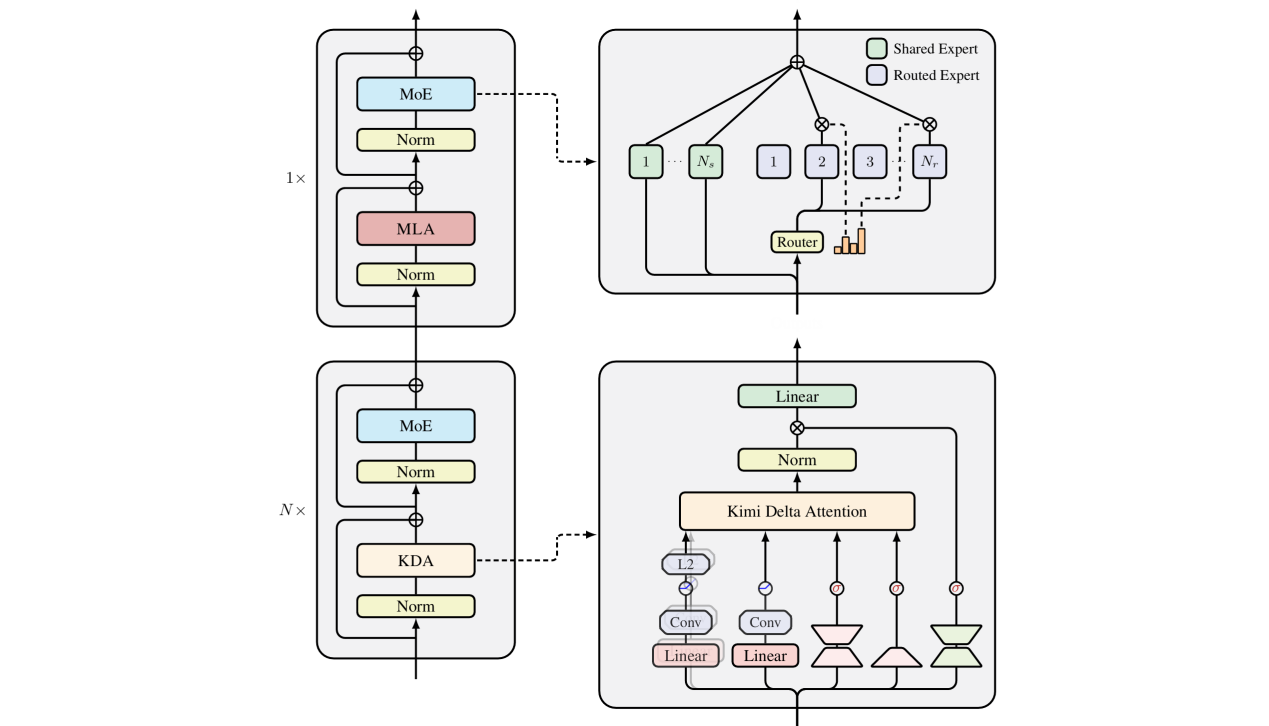
\includegraphics{images/image-0045.png}
\caption{Kimi Delta Attention 混合架构示意图}
\end{figure}

\hypertarget{ux56dbkdaux4e0ernn}{%
\subsection{四、KDA与RNN}\label{ux56dbkdaux4e0ernn}}

从原理上看，KDA本质上是一种RNN。那么，为什么KDA比传统RNN架构（如LSTM）效果更好呢？

\begin{enumerate}
\def\labelenumi{\arabic{enumi}.}
\item
  隐状态容量：LSTM的隐状态为d维向量，KDA的隐状态为d*d维矩阵。
\item
  能否利用GPU大规模并行训练
\end{enumerate}

在模型训练阶段，处理一个包含成千上万 token 的长文本时：

\begin{itemize}
\tightlist
\item
  LSTM 是被串行锁死的。LSTM 的状态更新公式是 \(h_t=\tanh(Wx_t+Uh_{t-1})\)，注意那个非线性激活函数 \(\tanh\)。它导致你必须等第 \(t-1\) 步的计算彻底完成，拿出确切的 \(h_{t-1}\) 后，才能开始算第 \(t\) 步。在拥有成千上万个流处理器的 GPU 面前，LSTM 只能排队一个一个算，GPU 算力被大量闲置。
\item
  KDA 是线性可并行的（Linear Recurrence）。忽略具体系数，KDA 的骨架公式可以写成：
\end{itemize}

\[
S_t=A_tS_{t-1}+V_t
\]

这个公式关于隐藏状态 \(S\) 是完全线性的（没有 \(\tanh\) 或 Sigmoid 阻挡）。根据矩阵乘法的结合律（Associativity），我们可以把时间序列展开：

\[
S_3=A_3(A_2S_1+V_2)+V_3=(A_3A_2)S_1+A_3V_2+V_3
\]

具体而言，对于推理的两个阶段：

A. 反馈集成阶段（Prefill 模式）：支持 token 间并行

当环境返回一段新的文本（例如搜索结果或环境状态变化）时，KDA 不需要像 RNN 那样一个 token 一个 token 地串行更新状态。

\begin{itemize}
\tightlist
\item
  Chunkwise-Parallel Algorithm：KDA 利用了线性注意力的结合律（Associativity）。通过数学变换，它可以将递推公式转化为块并行（Chunkwise）形式。
\item
  实现方式：如果环境反馈了 \(L\) 个 token，KDA 可以将这 \(L\) 个 token 作为一个``块''，在 GPU 上利用 Tensor Core 进行高并发的矩阵运算。一次运行即可处理完这 \(L\) 个 token，并直接得到最终的状态 \(S_{t+L}\)。
\item
  对比：传统模型处理新反馈时，KV Cache 的计算复杂度随总长度二次增长；而 KDA 处理新反馈的复杂度与总长度成线性关系。
\end{itemize}

B. 文本生成阶段（Decoding 模式）：单次运行生成，不可 token 间并行

当模型基于反馈开始生成新的回复（Action）时：

\begin{itemize}
\tightlist
\item
  单次运行：每生成一个新 token，确实只需要进行一次 \(O(1)\) 复杂度的前向传播。因为它只需读取上一步的状态 \(S_{t-1}\) 并计算 \(S_t\)，不需要重新扫描之前的全部上下文。
\item
  并行性限制：由于是自回归（Autoregressive）生成，token \(N+1\) 必须依赖 token \(N\) 生成后的状态。因此，在生成阶段无法实现 token 间并行（除非配合投机采样等技术）。
\end{itemize}

当然，这里如果环境反馈的序列较长，为了适配GPU，我们往往会进行分块处理，以一定量token作为一个块。

但总之，KDA可以运用FlashAttention这样的算子进行加速。

\begin{enumerate}
\def\labelenumi{\arabic{enumi}.}
\setcounter{enumi}{2}
\tightlist
\item
  数学本质：LSTM的更新是``启发式（Heuristic）''的：LSTM内部的遗忘门、输入门，是前人凭借直觉和实验凑出来的公式。网络只是隐式地学到一个``门限值''来决定保留什么、丢弃什么，它的本质是一个特征过滤器。
\end{enumerate}

KDA的更新是``第一性原理（First Principles）''的：如我们上一轮的推导，KDA的更新公式严格等价于在线梯度下降，即在线训练一个内部的线性回归模型。

面对新数据，KDA会算出预测误差，然后精准地沿着梯度的反方向修改记忆矩阵 \(S_t\)。这种严格的数学底座，使得KDA在处理复杂的逻辑推理和上下文学习（In-context Learning）时，拥有了碾压传统RNN的上限。

\hypertarget{ux4e94kdaux4e0eux5143ux5b66ux4e60}{%
\subsection{五、KDA与元学习}\label{ux4e94kdaux4e0eux5143ux5b66ux4e60}}

我们可以认为KDA是一种元学习（Meta-Learning）架构。在标准Transformer中，这种元学习是隐式的。而KDA将其变成了显式。

\begin{enumerate}
\def\labelenumi{\arabic{enumi}.}
\tightlist
\item
  外层循环：学习``如何在上下文中学习''
\end{enumerate}

在预训练阶段，我们在成千上万个 GPU 上使用标准的优化器（比如 AdamW），通过海量语料去更新 KDA 的物理参数，即用来生成 \(q,k,v\) 的投影权重 \(W_Q,W_K,W_V\)，以及遗忘门控 \(\alpha,\beta\)。

这些物理参数就是``元参数（Meta-parameters）''。AdamW 并没有教模型具体的知识，它是在教模型：

\begin{itemize}
\tightlist
\item
  遇到什么样的数据应该分配多大的学习率 \(\beta\)。
\item
  遇到什么特征应该开启遗忘门 \(\alpha\)。
\item
  如何从文本中提取最适合计算残差的 \(k\) 和 \(v\)。
\end{itemize}

\begin{enumerate}
\def\labelenumi{\arabic{enumi}.}
\setcounter{enumi}{1}
\tightlist
\item
  内层循环：在线梯度下降
\end{enumerate}

当模型部署后，你给它输入了一段长长的 Prompt。此时，物理参数（元参数）被冻结了，AdamW 优化器也下线了。

但是，KDA 内部的记忆矩阵 \(S_t\) 被激活了。随着你输入的数据一步步流入，KDA 严格按照外层循环教它的那套 Delta Rule，即在线梯度下降公式：

\[
S_t=S_{t-1}+\beta_tk_t\left(v_t-k_t^\top S_{t-1}\right)
\]

在 \(t\) 时刻的token输入KDA层时，隐状态根据 \(k_t\) 和 \(v_t\) 进行梯度下降更新，从 \(S_{t-1}\) 变为 \(S_t\)，带上了 \(t\) 时刻新的信息，但同时也已经在前 \(t-1\) 次梯度下降中保留了前 \(t-1\) 个token的信息（以先验形式存储在 \(S_{t-1}\) 中）。\(q_t\) 通过富含上下文 \(t\) 个token信息的 \(S_t\)，就实现了通过上下文学习来完成新的任务。

\begin{enumerate}
\def\labelenumi{\arabic{enumi}.}
\setcounter{enumi}{2}
\tightlist
\item
  其他参数（如embedding层、输入投影）：学习先验知识
\end{enumerate}

模型内部的embedding层、输入投影（MLP层）在预训练中记住了``秦始皇是哪一年称帝的''等人类世界的各种先验知识。这些先验知识被压入模型的这些参数，构成了模型极其庞大的高维特征子空间，确保模型输入被映射到符合其实际意义的向量，输入注意力层，如输入``苹果''时，MLP 瞬间把它映射到一个包含了``水果、红色、科技公司、牛顿''等无穷语义的特征坐标系中。

此外，对于输入的token，模型会根据先验参数判断是否需要启动上下文学习机制。如果问一个单纯的常识问题（比如``法国的首都是？''），模型根本不需要启动复杂的在下文梯度下降，它的MLP（先验知识）直接就能把``巴黎''的特征输出出来，此时 \(W_0\ne 0\) 而后续注意力层的 \(\Delta W\to 0\)。而对于模型在训练时没有见过的分布，会让 \(W_0\to 0\)（几乎没有先验，避免干扰上下文学习），而交给后续的 \(\Delta W\) 自主分析。

\hypertarget{ux53c2ux8003ux6587ux732e-137}{%
\subsection{参考文献}\label{ux53c2ux8003ux6587ux732e-137}}

\begin{itemize}
\tightlist
\item
  Moonshot AI. (2025). \href{https://arxiv.org/abs/2510.26692}{Kimi Linear: An Expressive, Efficient Attention Architecture}. arXiv:2510.26692.
\end{itemize}

\clearpage

\hypertarget{ux57faux4e8eux4e0aux4e0bux6587ux7684ux5143ux5f3aux5316ux5b66ux4e60ux8bbaux6587}{%
\section{基于上下文的元强化学习（论文）}\label{ux57faux4e8eux4e0aux4e0bux6587ux7684ux5143ux5f3aux5316ux5b66ux4e60ux8bbaux6587}}

\begin{quote}
本文是论文阅读笔记，内容代表对应论文方法或作者理解，不应直接视为领域共识或工程最佳实践。
\end{quote}

\hypertarget{ux4e00ux5143ux5f3aux5316ux5b66ux4e60ux7684ux57faux672cux601dux60f3}{%
\subsection{一、元强化学习的基本思想}\label{ux4e00ux5143ux5f3aux5316ux5b66ux4e60ux7684ux57faux672cux601dux60f3}}

元强化学习（Meta-RL）的目标不是让智能体掌握某一个具体任务，而是让智能体掌握一种学习策略。通过在大量的不同任务分布p(T)上进行元训练，从而在面对未见过的全新任务时，能够利用极少量的交互数据（Few-shot）实现快速适应。

一个强化学习任务 \(\mathcal{T}_i\) 可以被定义为一个马尔可夫决策过程（MDP）：

\[
\mathcal{T}_i = \{\mathcal{S}, \mathcal{A}, p_i(s_{t+1}\mid s_t,a_t), r_i(s_t,a_t), \gamma, H\}
\]

其中：

\begin{itemize}
\tightlist
\item
  \(\mathcal{S}, \mathcal{A}\)：状态空间和动作空间（通常假设跨任务共享）。
\item
  \(p_i(s_{t+1}\mid s_t,a_t)\)：状态转移概率（不同任务可能不同，如机器人的摩擦系数变化）。
\item
  \(r_i(s_t,a_t)\)：奖励函数（不同任务可能不同，如目标方向变化）。
\item
  \(H\)：时间视界（Horizon）。
\end{itemize}

Meta-RL 假设存在一个任务分布 \(p(\mathcal{T})\)。我们的目标是找到一组元参数（Meta-parameters）\(\theta\)，使得智能体在从分布中采样出的新任务 \(\mathcal{T}\sim p(\mathcal{T})\) 上，经过 \(K\) 步更新（或 \(K\) 条轨迹的适应）后，累积奖励最大化。

数学上，最大化目标函数 \(J(\theta)\)：

\[
\max_{\theta} J(\theta) =
\sum_{\mathcal{T}_i\sim p(\mathcal{T})}
\mathbb{E}_{\tau\sim p_{\mathcal{T}_i}(\tau\mid f_{\theta})}
[R(\tau)]
\]

其中，\(f_{\theta}\) 是由 \(\theta\) 参数化的适应过程（Adaptation Procedure），\(\tau\) 是轨迹。

\hypertarget{ux4e8cux57faux4e8eux4e0aux4e0bux6587ux7684ux5143ux5f3aux5316ux5b66ux4e60ux6982ux8ff0}{%
\subsection{二、基于上下文的元强化学习概述}\label{ux4e8cux57faux4e8eux4e0aux4e0bux6587ux7684ux5143ux5f3aux5316ux5b66ux4e60ux6982ux8ff0}}

我们已经知道，Transformer本质上等价于在上下文上作梯度下降，它本身就是一个持续学习的优化器。因此，对基于Transformer的大模型进行强化学习训练，本质上就是一个元学习过程，只不过没有显式地求二阶Hessian矩阵。因此，可以基于上下文设计元强化学习算法。

另一种思路是适应新任务本质上是一个部分可观察马尔可夫决策过程（POMDP）中的推断问题。在这种范式下，策略网络的权重在面对新任务时是固定不变的（不需要梯度下降）。相反，智能体会将过去的交互经验（状态、动作、奖励的序列）编码为一个隐变量（Latent Context/Representation）。策略网络只要通过将此上下文作为额外的输入条件，就可以隐式地改变其在不同任务中的行为。

下面介绍基于上下文的元强化学习算法。这些算法虽然在现在鲜有被直接提及，但却隐式地体现在现在的大模型中。

\hypertarget{ux4e09rl2}{%
\subsection{\texorpdfstring{三、RL\(^2\)}{三、RL\^{}2}}\label{ux4e09rl2}}

\hypertarget{ux4e00ux57faux672cux539fux7406ux548cux67b6ux6784}{%
\subsubsection{（一）基本原理和架构}\label{ux4e00ux57faux672cux539fux7406ux548cux67b6ux6784}}

在传统的单任务 RL 中，智能体面对环境只接收当前状态 \(s_t\)。但在 RL\(^2\) 中，为了让网络知道自己刚刚的``试错''是否有效，它必须拥有工作记忆（Working Memory）。

在传统的单任务 RL 中，智能体只接收当前状态 \(s_t\)。但在 RL\(^2\) 中，为了让网络知道自己刚才``试错''的结果，网络在时间步 \(t\) 的输入不仅包含当前状态 \(s_t\)，还包含上一步的动作 \(a_{t-1}\)、上一步的奖励 \(r_{t-1}\) 以及当前是否为回合结束的标志 \(d_{t-1}\)。

设输入向量为 \(x_t=(s_t,a_{t-1},r_{t-1},d_{t-1})\)。RL\(^2\) 使用循环神经网络（如 LSTM 或 GRU）来处理这个序列：

\[
h_t = f_{\theta}(x_t,h_{t-1})
\]

策略直接由隐藏状态生成：

\[
\pi_{\theta}(a_t\mid h_t)
\]

在这里，发生了两个时间尺度的学习：

\begin{itemize}
\tightlist
\item
  \textbf{慢速 RL（外环 Meta-training）}：也是权重更新的过程。在成千上万个不同的任务上，使用策略梯度算法（如 PPO 或 TRPO）来更新 RNN 的网络权重 \(\theta\)。
\item
  \textbf{快速 RL（内环 Adaptation）}：也是隐藏状态演化的过程。在面对一个全新任务时，权重 \(\theta\) 保持固定不动。智能体通过与环境交互，不断将 \((s,a,r)\) 喂给 RNN，RNN 的隐藏状态 \(h_t\) 随之更新。这个持续演化的 \(h_t\) 实际上充当了该任务的工作记忆（Working Memory）或信念状态（Belief State），从而瞬间改变了策略输出。
\end{itemize}

\hypertarget{ux4e8cux5de5ux4f5cux6d41-2}{%
\subsubsection{（二）工作流}\label{ux4e8cux5de5ux4f5cux6d41-2}}

\begin{enumerate}
\def\labelenumi{\arabic{enumi}.}
\tightlist
\item
  采样任务：从任务分布 \(p(\mathcal{T})\) 中采样一批任务。
\item
  构建序列（Trials）：对于每一个任务，执行 \(N\) 个回合（Episodes），这 \(N\) 个回合拼接成一个超长的序列（称为一个 Trial）。

  \begin{itemize}
  \tightlist
  \item
    关键点：在同一个 Trial（即同一个任务）内的不同 Episode 之间，RNN 的隐藏状态 \(h\) 不重置，而是保留下来跨回合传递。
  \item
    只有在切换到另一个全新任务时，隐藏状态 \(h\) 才会被清零。
  \end{itemize}
\item
  计算回报：累计整个 Trial 中所有回合的总奖励。
\item
  权重更新：将这些长序列数据输入到 TRPO 或 PPO 算法中，最大化期望总奖励，计算梯度并更新 RNN 权重 \(\theta\)。
\end{enumerate}

\hypertarget{ux4e09ux5b9eux73b0ux63a2ux7d22ux4e0eux5229ux7528ux5e73ux8861ux7684ux673aux5236}{%
\subsubsection{（三）实现探索与利用平衡的机制}\label{ux4e09ux5b9eux73b0ux63a2ux7d22ux4e0eux5229ux7528ux5e73ux8861ux7684ux673aux5236}}

RL\(^2\) 实现探索与利用的机制是完全隐式的（Implicit），由 RNN 在元训练中自己``悟''出来。

\begin{itemize}
\tightlist
\item
  \textbf{隐式的结构化探索}：假设任务是在迷宫中寻找一个随机放置的目标。在 Trial 的第 1 个回合（探索期），由于 \(h_0\) 是空的，RNN 会输出一些``扫描''策略（比如系统性地遍历每个房间）。在这个过程中，它虽然没得到奖励，但它记录了哪些地方去过（通过 \(x_t\) 中的 \(a\) 和 \(s\) 更新到 \(h\) 中）。
\item
  \textbf{向利用的自动切换}：一旦在某个时间步碰到了目标，收到了正奖励 \(r_{t-1}>0\)，这个信号就会输入给 RNN 并大幅改变隐藏状态 \(h_t\)。在随后的第 2 到第 \(N\) 个回合中（利用期），包含了``目标位置记忆''的隐藏状态 \(h_t\) 会直接驱使策略以最短路径走向目标。
\item
  \textbf{元目标驱动}：因为外环 PPO 优化的目标是最大化整个 Trial（\(N\) 个回合）的总收益，这就迫使 RNN 必须在最初的几个回合中采取高效率的试错行动（探索），以便在后续的回合中能够一直拿到最高分（利用）。
\end{itemize}

\hypertarget{ux56dbkimi-delta-attentionux4e2dux9690ux5f0fux7684rl2}{%
\subsubsection{\texorpdfstring{（四）Kimi Delta Attention中隐式的RL\(^2\)}{（四）Kimi Delta Attention中隐式的RL\^{}2}}\label{ux56dbkimi-delta-attentionux4e2dux9690ux5f0fux7684rl2}}

Kimi Delta Attention维护的线性注意力层本质上就可以视为RNN，从而本质上来说，在RL训练时这就是一个RL\(^2\) 算法：隐状态在每一个token生成（每一个epoch）后不会被清空，直到任务完成才会被重置。它的效果优于传统的RL\(^2\)，这是因为：

在原始的 RL\(^2\) 论文中，作者使用的是 LSTM 或 GRU，但这带来了严重的瓶颈，而 KDA 能有效解决这些痛点：

\begin{itemize}
\tightlist
\item
  \textbf{Meta-training 阶段的并行化加速}：LSTM 在训练（外环）时必须使用 BPTT（沿时间反向传播），只能一步步串行计算。而 KDA 作为线性注意力，在训练时可以通过\textbf{关联形式（Associative Form）}或\textbf{Chunkwise 并行计算机制}，像 Transformer 一样并行处理整个长序列。这极大地缩短了 Meta-RL 中极其漫长的外环训练时间。
\item
  \textbf{细粒度长程记忆控制}：传统 LSTM 的门控是粗粒度的。KDA 引入了通道级（Channel-wise）门控，让每个隐状态的维度独立决定记忆衰减。这意味着网络可以学到：用某些通道去锁死``目标全局坐标''这种绝对不能遗忘的信息（门控值接近 1），用另一些通道去记录``刚才走过哪个路口''的短期信息（快速衰减），从而在漫长的 Trial 中保持记忆的精度。
\end{itemize}

本质上来说，现在的Agentic RL就可以视为RL\(^2\) 的一种演进：

\begin{itemize}
\tightlist
\item
  \textbf{隐式到显式}：RL\(^2\) 将过去回合的试错经验压缩在 RNN 的隐状态 \(h_t\) 或 KDA 的 \(S_t\) 矩阵中；而 Agentic RLVR 将带有环境反馈的试错经验（``我刚才试了这段代码，服务器报了 404，所以我现在换个 API 试试''）以显式自然语言 Token 的形式写在了上下文窗口（KV Cache）中。
\item
  \textbf{学会探索（Learning to Explore）}：在 Agentic RLVR 的 Meta-training（外环权重更新）过程中，大模型逐渐学会了一种通用的、面对真实世界未知环境的探索策略。比如，当接到一个陌生任务时，它学会的第一步不再是盲目写代码，而是输出 \texttt{\textless{}action\textgreater{}\ ls\ -la\ \textless{}/action\textgreater{}} 或 \texttt{\textless{}action\textgreater{}\ cat\ README.md\ \textless{}/action\textgreater{}} 来探测环境状态。
\item
  \textbf{跨回合（Cross-episode）泛化}：只要环境的反馈被记录在上下文中，模型在测试阶段（权重 \(\theta\) 冻结）就能通过阅读前几步的真实报错 \((o_t)\)，利用注意力机制改变随后的动作 \((a_{t+1})\)，实现与真实世界的动态博弈和自适应修正。
\end{itemize}

\hypertarget{ux56dbpearl}{%
\subsection{四、PEARL}\label{ux56dbpearl}}

\hypertarget{ux4e00ux6838ux5fc3ux67b6ux6784}{%
\subsubsection{（一）核心架构}\label{ux4e00ux6838ux5fc3ux67b6ux6784}}

\begin{enumerate}
\def\labelenumi{\arabic{enumi}.}
\tightlist
\item
  \textbf{概率上下文编码器（Probabilistic Context Encoder）}
\end{enumerate}

在面对一个任务时，智能体会收集到一系列交互经验（Transitions），这些经验被称为上下文（Context），记为 \(c_{1:N}=\{(s_1,a_1,r_1,s'_1),\ldots,(s_N,a_N,r_N,s'_N)\}\)。

为了不像 RNN 那样严格依赖序列顺序，PEARL 设计了一个置换不变（Permutation-invariant）的编码器 \(q_{\phi}(\mathbf{z}\mid\mathbf{c})\)。它假设上下文中的每一次状态转移都是独立提供任务信息的。因此，编码器将每个转移元组 \((s,a,r,s')\) 通过多层感知机（MLP）映射为一个独立的高斯分布，然后将所有分布连乘起来，得到最终的后验隐变量分布：

\[
q_{\phi}(\mathbf{z}\mid\mathbf{c}_{1:N})
\propto
\prod_{n=1}^{N}
\mathcal{N}\left(f_{\phi}^{\mu}(c_n), f_{\phi}^{\Sigma}(c_n)\right)
\]

其中，\(\mathbf{z}\) 就是代表当前任务特征的连续隐变量，\(f_{\phi}^{\mu}\) 和 \(f_{\phi}^{\Sigma}\) 分别是输出均值和方差的网络。

\begin{enumerate}
\def\labelenumi{\arabic{enumi}.}
\setcounter{enumi}{1}
\tightlist
\item
  \textbf{条件 Actor-Critic 网络（Context-conditioned Actor-Critic）}
\end{enumerate}

PEARL 的底层强化学习算法通常基于 SAC（Soft Actor-Critic）。在推断出隐变量 \(z\) 后，\(z\) 会作为额外的输入，与当前状态 \(s\) 一起喂给策略网络和价值网络：

\begin{itemize}
\tightlist
\item
  Actor 网络（策略）：\(\pi_{\theta}(a\mid s,z)\)
\item
  Critic 网络（Q 值）：\(Q_{\theta}(s,a,z)\)
\end{itemize}

这意味着，网络权重 \(\theta\) 在不同任务之间是完全共享且固定的，策略的改变仅仅依赖于前向传播时输入的 \(z\) 的变化。

\hypertarget{ux4e8cux635fux5931ux51fdux6570}{%
\subsubsection{（二）损失函数}\label{ux4e8cux635fux5931ux51fdux6570}}

\begin{enumerate}
\def\labelenumi{\arabic{enumi}.}
\tightlist
\item
  \textbf{编码器的 KL 散度正则化}
\end{enumerate}

为了防止编码器对某一个具体的上下文序列过拟合，PEARL 强制后验分布 \(q_{\phi}(z\mid c)\) 逼近一个先验分布 \(p(z)\)（通常设为标准正态分布 \(\mathcal{N}(0,I)\)）。这通过最小化 KL 散度来实现：

\[
\mathcal{L}_{KL}(\phi)=\beta D_{KL}(q_{\phi}(z\mid c)\|p(z))
\]

其中 \(\beta\) 是调节信息瓶颈强度的超参数。

\begin{enumerate}
\def\labelenumi{\arabic{enumi}.}
\setcounter{enumi}{1}
\tightlist
\item
  \textbf{Critic 与 Actor 的损失函数}
\end{enumerate}

Critic 的更新目标是最小化引入了 \(z\) 的贝尔曼残差（Bellman Error）：

\[
\mathcal{L}_{critic}(\theta,\phi)=
\mathbb{E}_{(s,a,r,s')\sim\mathcal{B},z\sim q_{\phi}}
\left[
\left(
Q_{\theta}(s,a,z)-
(r+\gamma V_{\bar{\theta}}(s',z))
\right)^2
\right]
\]

这里的目标价值函数 \(V_{\bar{\theta}}\) 包含了 SAC 特有的熵最大化项（\(\alpha\) 为温度系数）：

\[
V_{\bar{\theta}}(s',z)=
\mathbb{E}_{a'\sim\pi_{\theta}}
\left[
Q_{\bar{\theta}}(s',a',z)-
\alpha\log\pi_{\theta}(a'\mid s',z)
\right]
\]

Actor 的更新目标则是最大化期望 Q 值并同时最大化策略熵：

\[
\mathcal{L}_{actor}(\theta)=
\mathbb{E}_{s\sim\mathcal{B},z\sim q_{\phi},a\sim\pi_{\theta}}
\left[
\alpha\log\pi_{\theta}(a\mid s,z)-
Q_{\theta}(s,a,z)
\right]
\]

在元训练期间，来自 Critic 损失的梯度会反向传播流经 \(z\)，从而更新编码器参数 \(\phi\)，迫使编码器提取那些``对预测奖励和价值最有用''的上下文信息。

\hypertarget{ux4e09ux8badux7ec3ux5de5ux4f5cux6d41-1}{%
\subsubsection{（三）训练工作流}\label{ux4e09ux8badux7ec3ux5de5ux4f5cux6d41-1}}

\begin{enumerate}
\def\labelenumi{\arabic{enumi}.}
\tightlist
\item
  \textbf{初始化}：初始化网络参数 \(\phi,\theta\)，为每个训练任务 \(\mathcal{T}_i\) 初始化空的重放缓冲区 \(\mathcal{B}_i\)。
\item
  \textbf{数据收集循环}：

  \begin{itemize}
  \tightlist
  \item
    从任务分布 \(p(\mathcal{T})\) 中采样一个任务 \(\mathcal{T}_i\)。
  \item
    初始化当前任务的上下文 \(c^i=\varnothing\)。
  \item
    \textbf{后验采样探索}：在每个 Episode 开始前，使用编码器计算分布并采样隐变量 \(\mathbf{z}\sim q_{\phi}(\mathbf{z}\mid\mathbf{c}^i)\)。在这个 Episode 内，\(\mathbf{z}\) 保持固定不变。
  \item
    智能体使用策略 \(\pi_{\theta}(a\mid s,\mathbf{z})\) 与环境交互，收集数据 \((s,a,r,s')\) 并将其存入缓冲区 \(\mathcal{B}_i\) 中。
  \item
    更新上下文 \(\mathbf{c}^i\leftarrow\mathbf{c}^i\cup\{(s,a,r,s')\}\)。
  \end{itemize}
\item
  \textbf{网络优化循环}：

  \begin{itemize}
  \tightlist
  \item
    随机采样一个批次（Batch）的任务。
  \item
    对于每个任务，从其对应的 \(\mathcal{B}_i\) 中随机抽取两组不相交的批次数据：

    \begin{itemize}
    \tightlist
    \item
      上下文批次 \(c^{batch}\)：送入编码器，推断出 \(z\) 的分布。
    \item
      RL 训练批次 \(b^{batch}\)：用于计算 SAC 损失。
    \end{itemize}
  \item
    从分布中采样 \(z\)，计算 \(\mathcal{L}_{critic}\)、\(\mathcal{L}_{actor}\) 和 \(\mathcal{L}_{KL}\)。
  \item
    使用梯度下降法联合更新参数 \(\phi\) 和 \(\theta\)。
  \end{itemize}
\end{enumerate}

\hypertarget{ux56dbagentic-rlux672cux8d28ux4e0aux662fpearlux7b49context-based-meta-rlux7b97ux6cd5ux7684ux6f14ux8fdb}{%
\subsubsection{（四）Agentic RL本质上是PEARL等Context-based Meta-RL算法的演进}\label{ux56dbagentic-rlux672cux8d28ux4e0aux662fpearlux7b49context-based-meta-rlux7b97ux6cd5ux7684ux6f14ux8fdb}}

无论是 PEARL 还是 Agentic RL，它们解决问题的核心数学公式是完全等价的：在测试阶段冻结网络权重 \(\theta\)，依靠不断增长的历史交互 \(C\)，来推断当前任务并输出最优动作 \(a_0\)。

\begin{itemize}
\tightlist
\item
  \textbf{Context-based Meta-RL（如 PEARL）}：策略网络的形式为 \(\pi_{\theta}(a_t\mid s_t,C_{1:t-1})\)。其中，上下文 \(C=\{(s_1,a_1,r_1,s_2),\ldots\}\) 是一堆交互经验。PEARL 使用一个编码器将 \(C\) 压缩成一个连续的隐变量 \(z\)，然后 Actor 根据 \(z\) 输出动作。
\item
  \textbf{Agentic RL（基于 LLM）}：策略网络（LLM）的形式为 \(\pi_{\theta}(a_t\mid\mathrm{Prompt}_t)\)。这里的 Prompt，就是上下文。它忠实地记录了历史轨迹：用户指令 \((s_0)\)、模型调用的工具代码 \((a_{1:t-1})\)、环境返回的终端报错或网页内容 \((s_{1:t})\)，以及客观奖励反馈 \((r_{1:t-1})\)。LLM 通过自注意力机制（Self-Attention）处理这段 Prompt，直接输出下一步的动作。
\end{itemize}

二者在数学上是同构的，只是状态载体发生了变化：从隐式、不可读的高维连续向量（\(z\) 或 \(h_t\)），变成了显式、人类可读的离散 Token 序列（KV Cache 中的文本）。

具体来说：

\begin{enumerate}
\def\labelenumi{\arabic{enumi}.}
\tightlist
\item
  \textbf{上下文记忆（Context c）}：

  \begin{itemize}
  \tightlist
  \item
    PEARL：记忆是一个无序的经验回放集合 \(\mathbf{c}=\{(s_i,a_i,r_i,s_{i+1})\}_{i=0}^{N}\)。
  \item
    LLM Agent：记忆是\textbf{上下文窗口（Context Window）}中拼接的 Token 序列（包含了 System Prompt、之前的动作命令、环境返回的真实终端报错以及步骤得分）。
  \end{itemize}
\item
  \textbf{任务推断与隐变量（Encoder \(q_{\phi}\) \& Latent \(z\)）}：

  \begin{itemize}
  \tightlist
  \item
    PEARL：使用基于 MLP 的概率编码器，输出一个连续的高斯分布隐变量 \(z\sim\mathcal{N}(\mu,\sigma^2)\)。\(z\) 代表了网络对当前陌生任务的``信念''。
  \item
    LLM Agent：LLM 的多头自注意力机制（Self-Attention）充当了天然的编码器，而深层的 KV Cache 构成了高维隐状态。更进一步，在带有显式推理的 Agent 中，模型通过生成``反思文本（Reflection / Chain-of-Thought）''，将对环境的推断显式地输出为了人类可读的 \(z\)。
  \end{itemize}
\item
  \textbf{策略网络（Actor \(\pi_{\theta}\)）}：

  \begin{itemize}
  \tightlist
  \item
    PEARL：策略是 \(\pi_{\theta}(a\mid s,z)\)，通过连续动作空间的强化学习算法更新。
  \item
    LLM Agent：策略是自回归语言建模头 \(\pi_{\theta}(a\mid\mathrm{Prompt},\mathrm{Reflection})\)，它在词表分布上进行温度采样，生成具体的 Python 代码或 Bash 命令。
  \end{itemize}
\end{enumerate}

虽然本质相同，但 Agentic RL 代表了 Meta-RL 演进的终极形态，它解决了传统 Meta-RL 的几个致命痛点：

\begin{enumerate}
\def\labelenumi{\arabic{enumi}.}
\tightlist
\item
  \textbf{极度泛化（从``白板''到``世界模型先验''）}：传统的 Meta-RL 是从零开始（Tabula Rasa）在特定环境中元训练的，它只能泛化到非常相似的同分布任务。而 Agentic LLM 已经通过海量互联网数据获得了极强的先验知识（世界模型）。它不需要再从头通过试错去学习``什么是 404 Error''或``什么是 Python 语法''，它可以直接调用预训练概念，实现真正意义上的 Zero-shot 或 Few-shot 跨域泛化。
\item
  \textbf{无损的长程信用分配}：无论是 RL\(^2\) 的 RNN 还是 PEARL 的高斯分布，在压缩几千步的 Trial 上下文时都会发生严重的信息丢失。而 Agentic RL 依托现代大模型的 KV Cache（或是你之前关注的 KDA 线性注意力机制），能够以极高的保真度保留极其久远的关键试错细节。
\item
  \textbf{显式的思维链（Chain-of-Thought）干预}：Agentic RL 可以在观测 \(o\) 和动作 \(a\) 之间，插入显式的推理想法。这种内部语言空间使得``探索逻辑''变得可解释，并且可以被外部规则（如 RLVR）进行精准的组内优势（Advantage）排序。
\end{enumerate}

\hypertarget{ux4e94llm-agent-with-meta-rllamer}{%
\subsection{五、LLM Agent with Meta-RL（LAMER）}\label{ux4e94llm-agent-with-meta-rllamer}}

\begin{enumerate}
\def\labelenumi{\arabic{enumi}.}
\tightlist
\item
  \textbf{跨回合训练框架（Cross-episode Training Framework）}
\end{enumerate}

LAMER 吸收了 RL\(^2\) 的宏观精髓，将环境交互的视距提升到了 Trial（试验）级别。

\begin{itemize}
\tightlist
\item
  一个完整的 Trial 包含多个独立的 Episode（回合）。
\item
  \textbf{奖励重塑}：算法优化的目标不再是单个回合的收益，而是跨回合折扣回报（Cross-episode discounted return）。
\end{itemize}

\[
J(\theta)=
\mathbb{E}_{\mathcal{T}\sim p(\mathcal{T}),\tau\sim\pi_{\theta}}
\left[
\sum_{k=1}^{K}\gamma^{k-1}R_k
\right]
\]

其中 \(K\) 是 Trial 内的总回合数，\(R_k\) 是第 \(k\) 个回合的总奖励。

\begin{itemize}
\tightlist
\item
  \textbf{探索的涌现}：这种严苛的奖励设计迫使大模型学会``放长线钓大鱼''。在早期的 Episode 中，模型会主动放弃眼前的安全低分，采取一些大概率会导致当前回合失败（但能探明环境机制或排除错误代码）的探索性动作。
\end{itemize}

\begin{enumerate}
\def\labelenumi{\arabic{enumi}.}
\setcounter{enumi}{1}
\tightlist
\item
  \textbf{结合自我反思的上下文策略适应（In-context Policy Adaptation via Self-Reflection）}
\end{enumerate}

这就是 PEARL 中生成推断隐变量 \(z\) 的最完美文本化体现。

LAMER 在测试（部署）阶段不进行任何网络参数的梯度更新。相反，在每一个 Episode 结束后（比如代码跑崩了），LAMER 会强制 LLM Agent 根据刚才积累的交互日志，生成一段纯文本的自我反思（Reflection）。

\begin{itemize}
\tightlist
\item
  这段反思文本会深入分析错误原因（例如：``我尝试向数组里 Append 字典，但引发了类型错误，因为接口需要 JSON 字符串''），并提出下一个回合的改进策略。
\item
  这个生成的 Reflection，会被作为强有力的先验上下文，直接 Prefix（前置拼接）到下一个 Episode \(k+1\) 的 Prompt 中。
\item
  依靠这种纯文本的演绎，Agent 的策略在下一个回合中发生了一次无需算力开销的 RL\(^2\) 飞跃。
\end{itemize}

\hypertarget{ux53c2ux8003ux6587ux732e-138}{%
\subsection{参考文献}\label{ux53c2ux8003ux6587ux732e-138}}

\begin{itemize}
\tightlist
\item
  Duan, Y., Schulman, J., Chen, X., Bartlett, P. L., Sutskever, I., \& Abbeel, P. (2016). \href{https://arxiv.org/abs/1611.02779}{RL\(^2\): Fast Reinforcement Learning via Slow Reinforcement Learning}. arXiv:1611.02779.
\item
  Rakelly, K., Zhou, A., Finn, C., Levine, S., \& Quillen, D. (2019). \href{https://arxiv.org/abs/1903.08254}{Efficient Off-Policy Meta-Reinforcement Learning via Probabilistic Context Variables}. ICML 2019.
\item
  Jiang, Y., Jiang, L., Teney, D., Moor, M., \& Brbic, M. (2025). \href{https://arxiv.org/abs/2512.16848}{Meta-RL Induces Exploration in Language Agents}. ICLR 2026.
\end{itemize}

\clearpage

\hypertarget{ux57faux4e8eux4e0aux4e0bux6587ux548cux957fux671fux8bb0ux5fc6ux7684ux6301ux7eedux5b66ux4e60ux8bbaux6587}{%
\section{基于上下文和长期记忆的持续学习（论文）}\label{ux57faux4e8eux4e0aux4e0bux6587ux548cux957fux671fux8bb0ux5fc6ux7684ux6301ux7eedux5b66ux4e60ux8bbaux6587}}

\begin{quote}
本文是论文阅读笔记，内容代表对应论文方法或作者理解，不应直接视为领域共识或工程最佳实践。
\end{quote}

\hypertarget{ux4e00ux591aux5c3aux5ea6ux8ba4ux77e5ux4ee5ml-masterux4e3aux4f8b}{%
\subsection{一、多尺度认知：以ML-Master为例}\label{ux4e00ux591aux5c3aux5ea6ux8ba4ux77e5ux4ee5ml-masterux4e3aux4f8b}}

\hypertarget{ux4e00ux6838ux5fc3ux67b6ux6784-1}{%
\subsubsection{（一）核心架构}\label{ux4e00ux6838ux5fc3ux67b6ux6784-1}}

HCC 将上下文分为三个层级，以应对不同时间尺度的认知需求：

\begin{itemize}
\tightlist
\item
  \(L_1\) 缓存：演进经验（Evolving Experience）

  \begin{itemize}
  \tightlist
  \item
    \textbf{作用}：作为智能体的工作记忆，保存当前执行所需的高保真原始轨迹（如当前的研究计划、代码补丁、终端报错和指标日志），用于即时调试和决策。
  \item
    \textbf{数学表达}：在当前阶段 \(p\) 的时间步 \(t\)，其缓存状态为 \(\mathcal{L}_1(t)=\mathcal{E}_{t_0-1}\cup\mathcal{P}_{p-1}\cup\mathcal{E}_{t_{p-1}+1:t}\)。其中 \(\mathcal{E}_{t_{p-1}:t}\) 是当前计划的原始执行轨迹。
  \end{itemize}
\item
  \(L_2\) 缓存：提炼知识（Refined Knowledge）

  \begin{itemize}
  \tightlist
  \item
    \textbf{作用}：作为中期战略记忆，存储从已完成的探索阶段中提炼出的稳定认知（如关键判断、实验洞察、精简的进度总结）。这让智能体在数十小时的探索中保持战略一致性，而无需携带冗长的执行日志。
  \item
    \textbf{数学表达}：\(\mathcal{L}_2(t)=\{\kappa_{t_{r-1}+1:t_r-1}\}_{r=1}^{p-1}\)，其中 \(\kappa\) 是通过大模型对原始事件片段进行提炼后得到的紧凑知识摘要。
  \end{itemize}
\item
  \(L_3\) 缓存：先验智慧（Prior Wisdom）

  \begin{itemize}
  \tightlist
  \item
    \textbf{作用}：作为长期记忆，存储跨任务可复用的抽象策略（如鲁棒的模型模板、数据处理流水线）。它使得智能体在面对新任务时能够``热启动''。
  \item
    \textbf{数学表达}：存储为嵌入-值对的集合 \(\mathcal{L}_3\triangleq(h_n,w_n)_{n=1}^{N}\)，其中 \(h_n\) 是检索键，\(w_n\) 是提炼出的任务级智慧文本。
  \end{itemize}
\end{itemize}

\hypertarget{ux4e8cux5de5ux4f5cux6d41-3}{%
\subsubsection{（二）工作流}\label{ux4e8cux5de5ux4f5cux6d41-3}}

为了在这三个缓存层之间动态流转信息，系统设计了严格的生命周期管理操作：

\begin{enumerate}
\def\labelenumi{\arabic{enumi}.}
\tightlist
\item
  \textbf{初始化与上下文预取（Context Prefetching）}：

  \begin{itemize}
  \tightlist
  \item
    给定新任务描述 \(d_{\tau}\)，系统计算其向量嵌入 \(q=E(d_{\tau})\)。
  \item
    通过余弦相似度阈值从 \(L_3\) 缓存中检索出相关的先验智慧：\(\Omega_{\tau}=\{w_n\mid(h_n,w_n)\in\mathcal{L}_3,\cos(q,h_n)>\delta\}\)。
  \item
    将检索到的智慧作为初始上下文，确保智能体在一个高起点的认知下开始探索。
  \end{itemize}
\item
  \textbf{执行与上下文命中（Context Hit）}：

  \begin{itemize}
  \tightlist
  \item
    在生成每一步的上下文时，系统优先从 \(L_1\) 提取当前活跃阶段的原始经验。
  \item
    对于过去已经完成的阶段，则退回到 \(L_2\) 提取高度浓缩的提炼知识。这有效防止了上下文饱和。
  \end{itemize}
\item
  \textbf{整合与上下文晋升（Context Promotion）}：

  \begin{itemize}
  \tightlist
  \item
    \textbf{阶段级晋升（\(P_1\)）}：当一个探索阶段结束时，智能体会利用 LLM 的总结能力，将 \(L_1\) 中的原始并行探索轨迹压缩成一个精炼的知识单元 \(\kappa_p\)，写入 \(L_2\)，并从 \(L_1\) 中清理掉对应的原始数据。
  \item
    \textbf{任务级晋升（\(P_2\)）}：当整个机器学习任务完成后，系统会从全局视角提取可复用的策略 \(w_{\tau}\)，并将其固化到 \(L_3\) 缓存中，供未来的任务检索使用。
  \end{itemize}
\end{enumerate}

\hypertarget{ux4e8cux8f7bux91cfux7ea7ux5206ux5c42ux8bb0ux5fc6lightmem}{%
\subsection{二、轻量级分层记忆：LightMem}\label{ux4e8cux8f7bux91cfux7ea7ux5206ux5c42ux8bb0ux5fc6lightmem}}

LightMem模仿人类的记忆系统，把记忆系统拆成三个轻量模块：

Light1：感官记忆（Sensory Memory），快速过滤无用信息、把输入压缩到``值得记''的部分，并进行主题切分。

具体做法：使用一个轻量压缩模型，在切分时避免``按窗口切''的粗暴做法，而是用注意力信号的峰值找到候选topic边界（见后），再用相邻片段的语义相似度做二次确认，取二者交集作为最终切分点，降低attention sink、注意力稀释等噪声影响导致的``伪峰值''。

怎么用注意力信号找到topic边界：让一个小参数量的语言模型先快速``读''一遍文本，当话题突变，可观察到新Token对旧话题Token的注意力权重 \(A_{i,j}\) 急剧下降，模型为了满足Softmax的归一化特性，会将注意力强制转移到新话题的起始Token上，这些位置就会形成注意力的局部峰值，通过找出峰值即可确定话题突变位置。

Light2：短时记忆（Short-Term Memory, STM），按主题把对话组织成结构化单元，降低总结调用次数，同时减少主题混杂。

具体做法：在拿到topic segments后，以 \texttt{\{topic,\ turns\}} 的结构送入STM buffer。达到token阈值时，才触发一次LLM总结，对每个topic生成更结构化的summary，并写入LTM。相比``每一轮都总结一次''，这样调用次数降低：总结不再是 \(N\) 次，而是按buffer触发的更少次数；输入被topic约束，不容易``把A主题的细节总结进B主题里''。

Light3：长时记忆（Long-Term Memory, LTM）+睡眠更新（Sleep-time Update），把昂贵的记忆更新从在线推理中``拿出来''，在离线并行地做去重、合并、修复与巩固。

具体做法：为了避免在test time将短时记忆转为长时记忆导致延时，系统在测试时新记忆条目到来时，直接插入LTM，不做复杂更新。离线阶段（sleep time）触发更新，对每个条目构建一个update queue（只允许``新的更新旧的''，即时间戳约束 \(t_j\ge t_i\)），然后把这些更新操作并行执行。

\begin{figure}[htbp]
\centering
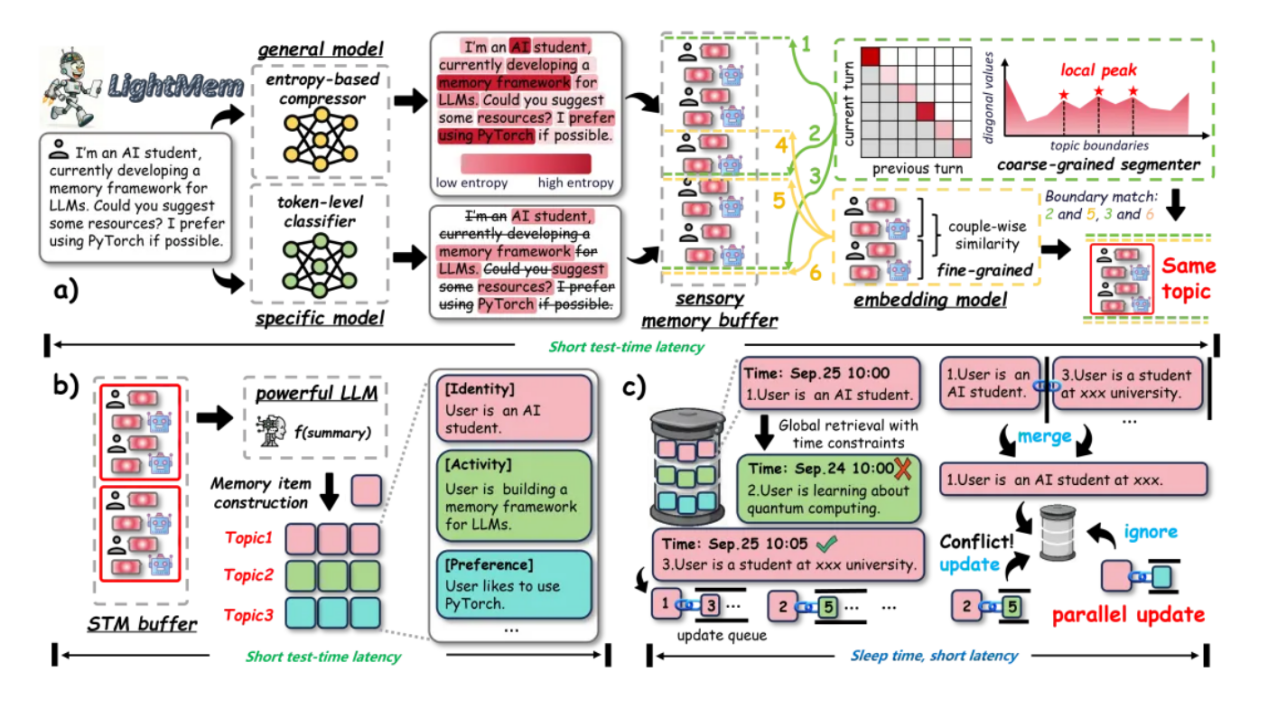
\includegraphics{images/image-0046.png}
\caption{LightMem 轻量级分层记忆系统示意图}
\end{figure}

\hypertarget{ux4e09ux751fux6210ux5668ux4e0eux8bb0ux5fc6ux7ba1ux7406ux667aux80fdux4f53ux534fux540cagentic-context-engineering}{%
\subsection{三、生成器与记忆管理智能体协同：Agentic Context Engineering}\label{ux4e09ux751fux6210ux5668ux4e0eux8bb0ux5fc6ux7ba1ux7406ux667aux80fdux4f53ux534fux540cagentic-context-engineering}}

\hypertarget{ux4e00ux6838ux5fc3ux67b6ux6784-2}{%
\subsubsection{（一）核心架构}\label{ux4e00ux6838ux5fc3ux67b6ux6784-2}}

\begin{enumerate}
\def\labelenumi{\arabic{enumi}.}
\item
  生成器（Generator）：接收新的查询并生成推理轨迹（包括有效策略和反复出现的陷阱） 。
\item
  反思器（Reflector）：批判这些生成的轨迹，从成功和错误中提取具体的经验教训，并可选择在多次迭代中进行提炼。同时，也给原有经验打上``有用''``有害''``中立''等标签。
\item
  策展人（Curator）：得到新的经验教训后，不重写上下文，而是将新的经验教训综合成紧凑的增量条目（delta entries）。这里的增量条目格式一般为``元数据（如ID，以及记录该条目被标记为``有用''或``有害''次数的计数器等）+内容（具体的策略、领域概念或常见错误等）''。
\item
  自动化脚本：得出增量条目后，将其确定性地合并到现有的上下文中。具体方式包括：（1）如果是一个带有新ID的新经验，直接追加到上下文列表的末尾；（2）如果是对某条旧规则的反馈，代码直接修改那条旧规则（比如把``有用''次数 +1）；（3）如果发现两条规则在向量空间相似度过高，就删除冗余。
\end{enumerate}

\hypertarget{ux4e8cux4e0aux4e0bux6587ux6e05ux7406ux673aux5236}{%
\subsubsection{（二）上下文清理机制}\label{ux4e8cux4e0aux4e0bux6587ux6e05ux7406ux673aux5236}}

作者认为，如果赋予大模型随意删除或重写整个上下文的权力，它往往会犯``简洁性偏见（Brevity Bias）''的毛病，为了追求简短和通用，大模型很容易把那些看起来有些繁琐但极其关键的``特定领域的启发式方法、工具使用指南或避坑细节''给丢弃掉。在ACE框架中，策展人（Curator）这个大模型角色本身并不负责直接发出``删除''指令，但整个系统确实存在一套机制来删除和清理原有经验，以防止上下文越积越多。

\begin{enumerate}
\def\labelenumi{\arabic{enumi}.}
\item
  语义去重与修剪：当策展人生成了新的经验条目后，底层的传统代码会计算所有经验条目的语义嵌入向量，若文本的语义上高度相似（即存在冗余），系统会自动执行去重并修剪掉多余的内容，用非LLM逻辑自动删除了重复的经验。
\item
  反思器的``有害''标记：在生成新经验之前，反思器（Reflector）会先对当前生成的轨迹进行复盘，并对上下文中被使用到的原有经验条目打上标签（helpful有用、harmful有害、neutral中立）。虽然策展人只负责输出需要添加的新洞察，但系统会根据反思器的标记来就地更新旧条目的计数器。这些指标可以帮助系统评估哪些经验是无效或起反作用的。
\item
  延迟提炼机制：修剪和提炼可以配置为主动进行（每次更新增量后都执行），也可以配置为延迟进行，即只有当上下文长度即将超出模型的上下文窗口限制时，才触发清理机制。
\end{enumerate}

\hypertarget{ux56dbux89c4ux5212ux4e0eux6267ux884cagentux7684ux8bb0ux5fc6ux5206ux79bbux5f0fux6301ux7eedux5b66ux4e60ux67b6ux6784}{%
\subsection{四、规划与执行Agent的记忆分离式持续学习架构}\label{ux56dbux89c4ux5212ux4e0eux6267ux884cagentux7684ux8bb0ux5fc6ux5206ux79bbux5f0fux6301ux7eedux5b66ux4e60ux67b6ux6784}}

\hypertarget{ux4e00ux57faux672cux601dux60f3-3}{%
\subsubsection{（一）基本思想}\label{ux4e00ux57faux672cux601dux60f3-3}}

在多智能体架构中，不同Agent负责规划、执行等，它们总结和需要使用的经验也会有所不同。因此，可将抽象的``规划逻辑''与具体的``执行技巧''分开提取、独立存储、分层检索。负责规划的Agent记忆（高层记忆）中往往是在给定总目标下，制定子目标、调度智能体等的方法和经验，负责执行的Agent记忆（底层记忆）中则是在具体子目标下执行的方法和经验。

\hypertarget{ux4e8cux8badux7ec3ux5de5ux4f5cux6d41}{%
\subsubsection{（二）训练工作流}\label{ux4e8cux8badux7ec3ux5de5ux4f5cux6d41}}

\begin{enumerate}
\def\labelenumi{\arabic{enumi}.}
\tightlist
\item
  \textbf{子目标推断（Subgoal Inference）}：
\end{enumerate}

给定一个任务 \(x\) 及其完整交互轨迹 \(\tau\)，利用大模型推断出该轨迹实际达成的一系列离散子目标序列 \(s_{1:N}\)。

\begin{enumerate}
\def\labelenumi{\arabic{enumi}.}
\setcounter{enumi}{1}
\tightlist
\item
  \textbf{子轨迹推断与分割（Subtrajectory Inference）}：
\end{enumerate}

根据推断出的子目标序列 \(s_{1:N}\)，将冗长、复杂的完整原始轨迹 \(\tau\) 在时间轴上切分为多个局部的子轨迹片段 \(\tau_{s_i}\)。这使得每一个子轨迹只专注于单一的子目标。

\begin{enumerate}
\def\labelenumi{\arabic{enumi}.}
\setcounter{enumi}{2}
\tightlist
\item
  \textbf{对比反思与洞察提取（Insight Extraction）}：
\end{enumerate}

这是最核心的``萃取''步骤。算法会同时对比同一任务下成功的轨迹 \(\tau^{+}\) 和失败的轨迹 \(\tau^{-}\)。

\begin{itemize}
\tightlist
\item
  \textbf{高层萃取}：对比成功的子目标序列和失败的序列，生成或更新全局的高层指导原则 \(I_{\mathrm{high}}\)（增加、修改、点赞或踩踏现有的 Rule）。
\item
  \textbf{底层萃取}：针对特定的子目标，对比成功和失败的子轨迹片段，提取出底层的避错原则 \(I_{\mathrm{low}}\)。
\end{itemize}

\begin{enumerate}
\def\labelenumi{\arabic{enumi}.}
\setcounter{enumi}{3}
\tightlist
\item
  \textbf{记忆单元组装与写入（Memory Unit Creation）}：
\end{enumerate}

将上述提取出的 \((x,s,I_{\mathrm{high}})\) 封装入 \(\mathcal{M}_{\mathrm{high}}\)；将 \((s_i,\tau_{s_i},I_{\mathrm{low}})\) 封装入 \(\mathcal{M}_{\mathrm{low}}\)。

\hypertarget{ux4e09ux6d4bux8bd5ux5de5ux4f5cux6d41}{%
\subsubsection{（三）测试工作流}\label{ux4e09ux6d4bux8bd5ux5de5ux4f5cux6d41}}

当面对一个全新的测试任务 \(x_{\mathrm{test}}\) 时，\(H^2R\) 采用``规划器（Planner）''与``执行器（Executor）''双重检索机制：

\begin{enumerate}
\def\labelenumi{\arabic{enumi}.}
\tightlist
\item
  \textbf{规划器检索（高层）}：
\end{enumerate}

规划器通过预训练的句向量编码器 \(\phi(\cdot)\) 计算当前任务与高层记忆库中历史任务的余弦相似度，检索出 Top-\(k\) 相关的规划记忆：

\[
\mathrm{sim}(x_{\mathrm{test}},x)=
\frac{\phi(x_{\mathrm{test}})\cdot\phi(x)}
{\|\phi(x_{\mathrm{test}})\|\|\phi(x)\|}
\]

结合检索到的经验，规划器将 \(x_{\mathrm{test}}\) 拆解为当前需要的子目标序列。

\begin{enumerate}
\def\labelenumi{\arabic{enumi}.}
\setcounter{enumi}{1}
\tightlist
\item
  \textbf{执行器检索（底层）}：
\end{enumerate}

对于规划器给出的当前子目标 \(s_{\mathrm{current}}\)，执行器以子目标为 Query，去底层记忆库 \(\mathcal{M}_{\mathrm{low}}\) 中进行相似度检索。根据检索到的底层交互技巧和子轨迹，执行器决定具体的原子动作（Atomic Actions），并判断该子目标是否已经完成或失效。

\hypertarget{ux4e94reactux7684ux6539ux8fdbremem}{%
\subsection{五、ReAct的改进：ReMem}\label{ux4e94reactux7684ux6539ux8fdbremem}}

在 ReMem 框架内，系统的整个决策循环被视为一个马尔可夫决策过程（Markov Decision Process）。

\begin{enumerate}
\def\labelenumi{\arabic{enumi}.}
\tightlist
\item
  \textbf{状态定义}：在时间步 \(t\) 且经过 \(n\) 次内部操作后，智能体的状态定义为 \(s_t^n=(x_t,M_t,o_t^{1:n-1})\)，即当前输入、当前记忆以及截至目前的推理轨迹 \(o_t\)。
\item
  \textbf{动作选择}：智能体在每一步需要从扩展的动作空间中选择一项指令：
\end{enumerate}

\[
a_t^n \in \{\mathrm{Think}, \mathrm{Act}, \mathrm{Refine}\}
\]

\begin{enumerate}
\def\labelenumi{\arabic{enumi}.}
\setcounter{enumi}{2}
\tightlist
\item
  \textbf{执行与状态转移}：智能体基于操作子 Agent 执行动作，输出结果 \(o_t^n=\mathrm{Agent}(x_t,M_t,a_t^n)\)。
\end{enumerate}

\begin{itemize}
\tightlist
\item
  \textbf{Think（思考）}：生成内部的推理思路，帮助分解当前复杂任务，为后续的策略规划提供指导。
\item
  \textbf{Refine（精炼）}：对自身的记忆网络执行高阶的元推理（Meta-reasoning）。在这个环节，模型会主动评估历史经验的利用率，召回成功的高价值策略，\textbf{剔除（Prune）}导致失败的噪音数据，并对 \(M_t\) 进行重新组织，从而为下一步提供更加纯净的高质量信息。
\item
  \textbf{Act（行动）}：在虚拟环境（如具身模拟器）中执行具体的命令，或直接向用户输出最终答案。
\end{itemize}

\hypertarget{ux516dux5176ux4ed6ux8defux5f84}{%
\subsection{六、其他路径}\label{ux516dux5176ux4ed6ux8defux5f84}}

\begin{enumerate}
\def\labelenumi{\arabic{enumi}.}
\item
  反思式学习：在推理后结合环境反馈自我批评，再把错误经验保留下来，主动从过去中抽取可复用的经验注入上下文。这可以做成跨回合、跨任务的经验积累机制。对代码、交互式任务、工具调用任务尤其有效，因为这类任务反馈信号明确。
\item
  技能库/程序库：把经验编译成模块化的可复用技能，即不只是记住一段自然语言经验，而是把成功推理/行动压缩成可调用的技能单元。每次成功完成任务后，提取可复用程序、子计划或策略模板，存成skill library，下次遇到相似任务时直接检索并组合技能。相比纯文本memory，技能库更结构化、更可执行，也更利于组合泛化。
\end{enumerate}

\hypertarget{ux4e03ux5c40ux9650ux6027}{%
\subsection{七、局限性}\label{ux4e03ux5c40ux9650ux6027}}

部分研究指出，长上下文ICL的提升很大程度上来自``检索相似样本''的适配，而不是``持久内化''。

此外，记忆确实能显著提升性能，但在稳定性和程序性经验重用方面依然很脆弱。在真实的非结构化业务场景中，基于提示词驱动的复杂Agent循环极其容易崩溃。如在在ReMem框架中，模型可能会错误地剪枝掉关键记忆，或在Think和Refine步骤中陷入无尽的自我怀疑和死循环，导致迟迟无法执行最终的Act。

\hypertarget{ux53c2ux8003ux6587ux732e-139}{%
\subsection{参考文献}\label{ux53c2ux8003ux6587ux732e-139}}

\begin{itemize}
\tightlist
\item
  Zhu, X., Cai, Y., Liu, Z., et al.~(2026). \href{https://arxiv.org/abs/2601.10402}{Toward Ultra-Long-Horizon Agentic Science: Cognitive Accumulation for Machine Learning Engineering}. arXiv:2601.10402.
\item
  Fang, J., Deng, X., Xu, H., et al.~(2025). \href{https://arxiv.org/abs/2510.18866}{LightMem: Lightweight and Efficient Memory-Augmented Generation}. ICLR 2026.
\item
  Zhang, Q., Hu, C., Upasani, S., et al.~(2025). \href{https://arxiv.org/abs/2510.04618}{Agentic Context Engineering: Evolving Contexts for Self-Improving Language Models}. ICLR 2026.
\item
  Ye, S., Yu, C., Ke, K., Xu, C., \& Wei, Y. (2025). \href{https://doi.org/10.1109/ICA67499.2025.00030}{H2R: Hierarchical Hindsight Reflection for Multi-Task LLM Agents}. ICA 2025.
\item
  Wei, T., Sachdeva, N., Coleman, B., et al.~(2025). \href{https://arxiv.org/abs/2511.20857}{Evo-Memory: Benchmarking LLM Agent Test-time Learning with Self-Evolving Memory}. arXiv:2511.20857.
\item
  Yao, S., Zhao, J., Yu, D., et al.~(2023). \href{https://arxiv.org/abs/2210.03629}{ReAct: Synergizing Reasoning and Acting in Language Models}. ICLR 2023.
\end{itemize}

\clearpage

\hypertarget{ux5229ux7528rlux8badux7ec3ux8bb0ux5fc6ux7ba1ux7406ux8bbaux6587}{%
\section{利用RL训练记忆管理（论文）}\label{ux5229ux7528rlux8badux7ec3ux8bb0ux5fc6ux7ba1ux7406ux8bbaux6587}}

\begin{quote}
本文是论文阅读笔记，内容代表对应论文方法或作者理解，不应直接视为领域共识或工程最佳实践。
\end{quote}

\hypertarget{ux4e00memory-r1}{%
\subsection{一、Memory-R1}\label{ux4e00memory-r1}}

\hypertarget{ux4e00ux6838ux5fc3ux67b6ux6784-3}{%
\subsubsection{（一）核心架构}\label{ux4e00ux6838ux5fc3ux67b6ux6784-3}}

Memory-R1 框架由两个协同工作的智能体组成：\textbf{Memory Manager（内存管理器）} 和 \textbf{Answer Agent（问答智能体）}。它们都通过强化学习（PPO 或 GRPO）进行微调，以最终的问答准确率作为奖励信号。

\begin{enumerate}
\def\labelenumi{\arabic{enumi}.}
\tightlist
\item
  \textbf{Memory Manager：从静态存储到动态的增删改查}
\end{enumerate}

传统的记忆系统往往缺乏学习机制来决定信息的去留。Memory Manager 将记忆管理建模为一个结构化的动作选择问题：当从新对话中提取出信息 \(x\) 并检索到现有记忆库 \(\mathcal{M}_{old}\) 时，策略网络 \(\pi_\theta\) 会输出四个操作之一（\texttt{ADD}、\texttt{UPDATE}、\texttt{DELETE}、\texttt{NOOP}）以及更新后的内容 \(m'\)：

\[
(o,m') \sim \pi_\theta(\cdot|x,\mathcal{M}_{old})
\]

\begin{enumerate}
\def\labelenumi{\arabic{enumi}.}
\setcounter{enumi}{1}
\tightlist
\item
  \textbf{Answer Agent：基于强化学习的记忆蒸馏（Memory Distillation）}
\end{enumerate}

面对 RAG 召回的大量 context 块，如果直接``喂''给生成模型，往往会导致答案偏误。Answer Agent 的任务是在生成答案前，先对检索到的 60 条候选记忆进行``蒸馏''（过滤去噪）。

这种蒸馏策略不是基于简单的向量相似度，而是通过强化学习、以结果为导向训练出来的。它确保模型只关注能推导出正确答案的核心信息。

\hypertarget{ux4e8cux5de5ux7a0bux96beux70b9}{%
\subsubsection{（二）工程难点}\label{ux4e8cux5de5ux7a0bux96beux70b9}}

\begin{enumerate}
\def\labelenumi{\arabic{enumi}.}
\tightlist
\item
  \textbf{奖励信号（Reward Signal）的极其稀疏与评估悖论}
\end{enumerate}

在论文中，强化学习的奖励函数 \(R_{answer}\) 是基于``精确匹配''（Exact Match, EM）计算的。这在标准化的学术数据集（如 LoCoMo）中很完美。但在真实的工业场景（如开放式问答、代码辅助、复杂业务查询）中，根本不存在唯一的 \(y_{gold}\)（标准答案）。

如果使用 LLM-as-a-Judge（让大模型当裁判）来给奖励，不仅计算成本极其高昂，而且法官模型往往偏好冗长的废话（Verbosity bias）。论文中也承认，使用基于 Judge 的奖励模型反而会导致 F1 和 BLEU-1 分数大幅下降。

\begin{enumerate}
\def\labelenumi{\arabic{enumi}.}
\setcounter{enumi}{1}
\tightlist
\item
  \textbf{状态空间爆炸与误差级联（Error Cascading）}
\end{enumerate}

数据库的 CRUD 操作是确定性的，而基于 LLM 策略生成的 \texttt{UPDATE} 或 \texttt{DELETE} 操作是概率性的。在漫长的用户交互周期中，如果 Memory Manager 在某一天错误地 \texttt{DELETE} 了一条核心业务逻辑或个人偏好，这种信息丢失是不可逆的。随着记忆库的膨胀，错误的累积会导致系统状态（State）彻底崩溃。

\begin{enumerate}
\def\labelenumi{\arabic{enumi}.}
\setcounter{enumi}{2}
\tightlist
\item
  \textbf{多智能体强化学习（MARL）的联合训练极不稳定}
\end{enumerate}

仔细阅读论文的 Limitation 会发现一个关键细节：\textbf{Memory Manager 和 Answer Agent 是分开独立训练的}。在训练 Manager 时，冻结 Answer Agent；在训练 Answer 时，冻结 Manager。

在一个真正的工业级在线系统中，如果让两个智能体端到端地同时在线强化学习（End-to-end MARL），由于环境的非平稳性（Non-stationarity）和奖励的极度延迟，损失函数的地形（Loss landscape）会变得极度非凸且混乱，这在工程上极难收敛。

\begin{enumerate}
\def\labelenumi{\arabic{enumi}.}
\setcounter{enumi}{3}
\tightlist
\item
  \textbf{基础设施的改造成本过高}
\end{enumerate}

现有的工业级 RAG 架构（如各种大厂的 AI 搜索产品）主要依赖于``无状态 LLM + 静态向量数据库''的解耦模式。计算层和存储层分离，易于弹性扩容。而 Memory-R1 这种机制要求为每一个独立用户/Session 实时维护并计算一个动态读写的记忆空间，并且在每次信息写入时都要运行一次大模型的推理（甚至要经过策略网络的采样）。这会带来难以承受的并发计算成本和架构复杂度。

\hypertarget{ux4e8cretroagent}{%
\subsection{二、RetroAgent}\label{ux4e8cretroagent}}

当前基于 LLM 的智能体通常使用标准强化学习算法进行训练，这些方法过度依赖环境提供的``外部任务成功奖励''（Extrinsic Rewards）。这种机制存在两个主要缺陷：

\begin{itemize}
\tightlist
\item
  \textbf{探索不足导致次优策略}：智能体一旦偶然发现一种可行的动作序列，往往会过度利用该策略，停止探索其他可能的更优解。
\item
  \textbf{经验隐式存储导致泛化能力差}：智能体在交互中积累的经验被隐式地埋藏在模型参数中，在面对后续决策时，很难显式地提取并复用相关的历史教训。
\end{itemize}

为了突破这一瓶颈，作者受到人类``事后自我反思''（Retrospective Self-improvement）能力的启发，提出了 RETROAGENT 框架。

\hypertarget{ux4e00ux6838ux5fc3ux601dux60f3-11}{%
\subsubsection{（一）核心思想}\label{ux4e00ux6838ux5fc3ux601dux60f3-11}}

\begin{enumerate}
\def\labelenumi{\arabic{enumi}.}
\item
  通过原生RL让主Agent原生学会总结文字经验的方法，不是纯套框架。
\item
  通过UCB算法、同组内部分探索不注入经验等方法，避免主Agent被完全``困''在高价值经验中导致结果反而变差。
\item
  在主Agent之外，还有一个评估Agent，负责结合``潜力''给出密集的标量反馈，鼓励探索``改进一小步''。
\end{enumerate}

\hypertarget{ux4e8cux5185ux5728ux53cdux9988ux673aux5236}{%
\subsubsection{（二）内在反馈机制}\label{ux4e8cux5185ux5728ux53cdux9988ux673aux5236}}

\begin{enumerate}
\def\labelenumi{\arabic{enumi}.}
\tightlist
\item
  数值反馈
\end{enumerate}

数值反馈可在RL阶段作为奖励函数的一部分，以鼓励探索新方式\&将新技能吸收入经验。

该反馈用于衡量智能体在子任务上的增量进展，并将其转化为数值奖励，以鼓励那些尚未获得最终成功但极具潜力的探索行为。

\begin{itemize}
\tightlist
\item
  \textbf{反思与评估}：智能体通过评估函数获得一个介于 0 到 1 之间的潜力分数 \(\phi(x,\tau)\)，用于量化当前轨迹对于子任务的完成度。
\item
  \textbf{能力进化奖励计算}：系统维护一个历史最佳表现基线 \(\Phi_x\)（由过往最高组平均成功率得出）。内在奖励 \(R^{int}\) 只有在当前潜力分数超越该基线时才会发放：
\end{itemize}

\[
R^{int} := \max(0,\phi(x,\tau)-\Phi_x)
\]

\begin{itemize}
\tightlist
\item
  \textbf{基线更新}：随后使用当前 rollout 组的平均成功率 \(\bar{I}^{ext}\) 更新基线，确保优化过程建立在稳健的历史表现之上：
\end{itemize}

\[
\Phi_x := \max(\Phi_x,\bar{I}^{ext})
\]

这部分看似不直接记下经验，实则``押注''即将带来高价值的经验，将参数朝其方向优化。

\begin{enumerate}
\def\labelenumi{\arabic{enumi}.}
\setcounter{enumi}{1}
\tightlist
\item
  语言反馈
\end{enumerate}

语言反馈在RL和推理阶段均可存取，每轮回答完成后，都生成一段语言反思存入缓冲区，此后一直记录该反思被调用的次数及自身在对应任务的成功率。而每轮回答前，模型也要参考缓冲区的经验回放，取时用UCB以保持一定的探索。

由于纯数值奖励缺乏语义丰富度，RETROAGENT 进一步从成功或失败的轨迹中提取自然语言形式的``教训''（Lessons），存储在外部记忆库 \(\mathcal{B}\) 中。

为了高效复用这些经验，论文提出了一种 \textbf{SimUtil-UCB}（相似度与效用感知的置信上限）记忆检索策略，它综合平衡了以下三个维度：

\begin{itemize}
\tightlist
\item
  \textbf{语义相关性（Semantic Relevance）}：使用余弦相似度 \(s_{rel}(x,x_i)\) 确保检索到的教训与当前任务高度相关。
\item
  \textbf{反思效用（Reflection Utility）}：根据教训在历史使用中带来的任务成功率，使用指数移动平均更新其效用得分 \(u_i\)。
\item
  \textbf{探索覆盖率（Exploration Coverage）}：为防止智能体陷入``信息茧房''（反复使用少数几个教训），引入 UCB 探索项。结合效用得分的公式为：
\end{itemize}

\[
u_{UCB}^{(i)} := u_i + \kappa\sqrt{\frac{\ln N}{n_i}}
\]

\begin{itemize}
\tightlist
\item
  \textbf{综合检索得分}：最终通过权重 \(\alpha\) 平衡相关性与效用：
\end{itemize}

\[
S(b_i|x) := \alpha s_{rel}(x,x_i) + (1-\alpha)u_{UCB}^{(i)}
\]

\hypertarget{ux4e09ux8badux7ec3ux5de5ux4f5cux6d41-2}{%
\subsubsection{（三）训练工作流}\label{ux4e09ux8badux7ec3ux5de5ux4f5cux6d41-2}}

\begin{enumerate}
\def\labelenumi{\arabic{enumi}.}
\tightlist
\item
  \textbf{经验注入与轨迹生成}：给定任务指令 \(x\)，系统生成 \(N\) 条轨迹。其中一半由基础策略独立探索生成，另一半由结合了 SimUtil-UCB 检索结果的``记忆增强策略''生成，以此兼顾经验利用与新知探索。
\item
  \textbf{事后自我反思}：回合结束后，智能体调用反思函数 \(f_{reflect}(\tau)\) 分析生成的轨迹，输出包含潜力分数 \(\phi(x,\tau)\)、成功率预测 \(c\) 以及自然语言教训 \(m\) 的反思元组。
\item
  \textbf{计算混合奖励}：环境提供的稀疏外部奖励 \(R^{ext}\) 被均匀分配到每个时间步，随后与内在的数值奖励 \(R^{int}\) 结合，形成复合奖励信号。
\item
  \textbf{记忆库更新}：将步骤 2 中提取的自然语言教训 \(m\) 连同其实用性数据写入记忆库 \(\mathcal{B}\) 中，供未来步骤检索。
\item
  \textbf{策略联合优化}：基于计算出的复合奖励和优势函数，使用 RL 算法更新模型参数。
\end{enumerate}

\hypertarget{ux56dbux76eeux6807ux51fdux6570}{%
\subsubsection{（四）目标函数}\label{ux56dbux76eeux6807ux51fdux6570}}

\begin{enumerate}
\def\labelenumi{\arabic{enumi}.}
\tightlist
\item
  主Agent的优化目标
\end{enumerate}

结合了外在与内在双重反馈的复合目标函数，计算基于组的相对优势 \(\hat{A}^{(i)}\)，并通过 PPO 风格的截断损失和 KL 散度正则化进行优化：

\[
\mathbb{E}\left[
\frac{1}{N}\sum_{i=1}^{N}
\frac{1}{T_i}\sum_{t=0}^{T_i-1}
\frac{1}{|a_t^{(i)}|}\sum_{j=1}^{|a_t^{(i)}|}
\left(
\mathcal{L}_{t,j}^{clip}(\theta,\hat{A}^{(i)})
-\beta D_{KL}\left[\pi_\theta(\cdot|s_t^{(i)})\|\pi_{ref}(\cdot|s_t^{(i)})\right]
\right)
\right]
\]

\begin{enumerate}
\def\labelenumi{\arabic{enumi}.}
\setcounter{enumi}{1}
\tightlist
\item
  评估Agent的优化目标
\end{enumerate}

我们无法直接通过潜力分数来优化评估Agent。因此，我们只能保证评估Agent的客观性和准确性。我们让评估Agent对自己刚才那趟轨迹是否最终完成了目标进行二元判断，然后确认实际情况与其判断是否一致，如果一致则给出奖励：

\[
R^{reflect} := R^{ext}\cdot \mathbb{I}(c=I^{ext})
\]

随后使用 REINFORCE 算法优化反思策略 \(\varphi_\theta\)：

\[
\mathcal{J}_{Reflection}(\theta)
= \mathbb{E}\left[
\frac{1}{N}\sum_{i=1}^{N}
\frac{1}{|z^{(i)}|}
\sum_{j=1}^{|z^{(i)}|}
\log \varphi_\theta(z_j^{(i)}|\tau^{(i)},z_{<j}^{(i)})
\cdot R^{reflect,(i)}
\right]
\]

为什么优化 \(c\) 对优化评估潜力分数的能力有用？

这是因为REINFORCE算法``一人得道，鸡犬升天''的特性，把答案token的奖励分散在了过程的每一个token上：

\[
\mathcal{J}_{Reflection}(\theta)
= \mathbb{E}\left[
\cdots
\sum_{j=1}^{|z^{(i)}|}
\log \varphi_\theta(z_j^{(i)}|\tau^{(i)},z_{<j}^{(i)})
\cdot R^{reflect,(i)}
\right]
\]

这在直觉上意味着：

\begin{itemize}
\tightlist
\item
  \(c\) 是这道题的\textbf{最终答案}。
\item
  \(\phi(x,\tau)\) 和文字教训 \(m\) 是得出答案前的\textbf{中间推导步骤（思考过程）}。
\item
  老师（环境）为了节省算力或因为缺乏中间步骤的标准答案，\textbf{只根据最终答案 \(c\) 对不对来给分}。
\item
  但是，通过策略梯度下降，只要最终答案 \(c\) 对了，模型就会认为``我刚才写的那一长串推导步骤 \(\phi(x,\tau)\) 也是极其合理的''，从而在参数更新时，把生成那段高质量 \(\phi(x,\tau)\) 的概率也一并放大了。
\end{itemize}

\hypertarget{ux53c2ux8003ux6587ux732e-140}{%
\subsection{参考文献}\label{ux53c2ux8003ux6587ux732e-140}}

\begin{itemize}
\tightlist
\item
  Yan, X., et al.~(2025). \href{https://arxiv.org/abs/2508.19828}{Memory-R1: Enhancing Large Language Model Agents to Manage and Utilize Memories via Reinforcement Learning}. arXiv:2508.19828.
\item
  Zhang, X., Liu, Z., Zhang, Y., Hu, X., \& Shao, W. (2026). \href{https://arxiv.org/abs/2603.08561}{RetroAgent: From Solving to Evolving via Retrospective Dual Intrinsic Feedback}. arXiv:2603.08561.
\end{itemize}

\clearpage

\hypertarget{hymbaux5934ux7ea7ux522bux6df7ux5408ux6ce8ux610fux529bux8bbaux6587}{%
\section{Hymba：头级别混合注意力（论文）}\label{hymbaux5934ux7ea7ux522bux6df7ux5408ux6ce8ux610fux529bux8bbaux6587}}

\begin{quote}
本文是论文阅读笔记，内容代表对应论文方法或作者理解，不应直接视为领域共识或工程最佳实践。
\end{quote}

\hypertarget{ux4e00ux6838ux5fc3ux67b6ux6784-4}{%
\subsection{一、核心架构}\label{ux4e00ux6838ux5fc3ux67b6ux6784-4}}

Nvidia提出，可以在同一个Attention层内，让一部分注意力头（Heads）执行精准的Full Attention，另一部分头执行类似Linear Attention的状态空间更新，最后把所有头的输出Concatenate或者相加在一起。

和Kimi``3层Linear接1层Attention''的串行堆叠不同，Hymba在同一个网络层内，直接让两种不同的``头''并行工作：Attention Heads负责精确召回，就像人类的``快照记忆''，精准但极其耗费系统资源，其计算和内存复杂度均为O(N\^{}2)；Mamba Heads就像人类的``长期记忆''，能以O(N)的线性复杂度纵观全局，但难以精准定位细节。

输入序列同时进入这两种头。两者同时处理相同的Token，提取不同的特征，最后在当前层内将输出的隐状态进行拼接和融合。这就确保了长程信息的无损保留，同时避免了串行堆叠带来的``信息断层''。

\hypertarget{ux4e8cmeta-tokensux5143ux6807ux8bb0}{%
\subsection{二、Meta Tokens（元标记）}\label{ux4e8cmeta-tokensux5143ux6807ux8bb0}}

Hymba在所有输入的开头固定插入128个可学习的Embedding。这解决了纯Attention模型中的``Attention Sinks''（注意力黑洞，即模型会被迫把大量注意力浪费在第一个BOS Token上）问题。Meta Tokens提前吸收了这些冗余的注意力，让后续真正的输入Token能够更专注地相互交互。

\hypertarget{ux4e09hymbaux8fd0ux7528ux4e8eux5927ux6a21ux578bux7684ux969cux788d}{%
\subsection{三、Hymba运用于大模型的障碍}\label{ux4e09hymbaux8fd0ux7528ux4e8eux5927ux6a21ux578bux7684ux969cux788d}}

\begin{enumerate}
\def\labelenumi{\arabic{enumi}.}
\item
  计算密度的不平衡：Linear Attention的计算是内存密集型的（Memory-bound），而Full Attention是计算密集型的（Compute-bound）。在 1.5B 的体量下，单卡运行，不同架构分支（密集计算的Attention和访存密集的Mamba）的算子调度不平衡问题可以通过底层重写（如NVIDIA FlexAttention）来压制。但如果放大到百亿、千亿参数规模，跨多个GPU节点进行Mamba隐状态和Attention状态的混合并行通信，系统复杂度会呈指数级上升，为了等并行分支同步，极其容易造成GPU计算单元的空转等待。
\item
  KV Cache的碎片化：按层堆叠（比如3层线性接1层全注意力）在工程实现上极其干净，全注意力层集中管理巨大的KV Cache，线性层几乎不需要Cache。而如果在同一层内做门控或旁路，系统需要为每一层都维护复杂的动态Cache路由。
\end{enumerate}

\hypertarget{ux53c2ux8003ux6587ux732e-141}{%
\subsection{参考文献}\label{ux53c2ux8003ux6587ux732e-141}}

\begin{itemize}
\tightlist
\item
  Dong, X., Fu, Y., Diao, S., et al.~(2025). \href{https://arxiv.org/abs/2411.13676}{Hymba: A Hybrid-head Architecture for Small Language Models}. ICLR 2025.
\end{itemize}

\clearpage

\hypertarget{memory-sparse-attentionux8bbaux6587}{%
\section{Memory Sparse Attention（论文）}\label{memory-sparse-attentionux8bbaux6587}}

\begin{quote}
本文是论文阅读笔记，内容代表对应论文方法或作者理解，不应直接视为领域共识或工程最佳实践。
\end{quote}

Memory Sparse Attention（MSA）是盛大集团研究团队提出的一种长上下文处理方法，将文档检索融入了注意力机制之中。

\hypertarget{ux4e00ux6838ux5fc3ux67b6ux6784-5}{%
\subsection{一、核心架构}\label{ux4e00ux6838ux5fc3ux67b6ux6784-5}}

\hypertarget{ux4e00ux57faux4e8eux6587ux6863ux68c0ux7d22ux7684ux7a00ux758fux6ce8ux610fux529b}{%
\subsubsection{（一）基于文档检索的稀疏注意力}\label{ux4e00ux57faux4e8eux6587ux6863ux68c0ux7d22ux7684ux7a00ux758fux6ce8ux610fux529b}}

对于每个文档 \(d_i\) 及其隐藏状态 \(H_i\)，除了生成标准的键值矩阵外，模型引入了一个路由器投影器（Router Projector）来生成专门的路由键矩阵 \(K_i^{R}\)：

\[
K_{i,h}=H_iW_K^h,\quad V_{i,h}=H_iW_V^h,\quad K_{i,h}^{R}=H_iW_{K^R}^h
\]

为了降低内存和检索复杂度，模型将文档分割为固定长度的块（Chunks），并使用均值池化（mean pooling，记为 \(\phi\)）进行压缩，得到 \(\bar{K}_{i,h}\)、\(\bar{V}_{i,h}\) 和 \(\bar{K}_{i,h}^{R}\)。查询（Query）也通过类似方式生成路由查询 \(Q_{q,h}^{R}\)，通过余弦相似度计算查询与每个文档块的相关性得分 \(S_{ij}\)：

\[
S_{ij}=\max_{\text{token }t}\left(\mathrm{mean}_{\text{head }h}\big(\cos(Q_{q,h}^{R},\bar{K}_{ij,h}^{R})\big)\right)
\]

然后取文档中得分最高的块作为文档得分，并选取 Top-k 个文档的压缩 KV 矩阵，拼接在局部缓存之前供后续的自回归生成使用。

和 RAG 的不同点：RAG 基于模型无关的语义相似度（例如余弦相似度），这与模型内部进行下一 Token 预测的生成目标之间存在一条``优化鸿沟''；MSA 则内置于模型中，生成 Q、K、V 所需的 \(W_Q\)、\(W_K\)、\(W_V\) 矩阵均为模型内置的矩阵，就可以将检索过程转变为可以端到端联合优化的注意力机制。

\hypertarget{ux4e8cux53ccux5c42ux4f4dux7f6eux7f16ux7801}{%
\subsubsection{（二）双层位置编码}\label{ux4e8cux53ccux5c42ux4f4dux7f6eux7f16ux7801}}

长文本模型常面临``短文本训练、长文本推理（train-on-short, infer-on-long）''的位置编码偏移问题。

\begin{itemize}
\tightlist
\item
  \textbf{文档级 RoPE（Doc-wise RoPE）}：MSA 为记忆库中的每个文档分配独立的起始位置 ID（从 \(0\) 开始），使位置语义与文档总数解耦，从而实现了极强的长度外推能力。
\item
  \textbf{全局 RoPE（Global RoPE）}：针对活跃的上下文（用户查询和生成的回答），其位置 ID 顺延于被检索文档的数量（从 \(k\) 开始），以保留连贯生成所需的因果依赖性。
\end{itemize}

\hypertarget{ux4e8cux5de5ux4f5cux6d41-4}{%
\subsection{二、工作流}\label{ux4e8cux5de5ux4f5cux6d41-4}}

\hypertarget{ux4e00ux7aefux5230ux7aefux8badux7ec3ux9636ux6bb5}{%
\subsubsection{（一）端到端训练阶段}\label{ux4e00ux7aefux5230ux7aefux8badux7ec3ux9636ux6bb5}}

\begin{itemize}
\tightlist
\item
  \textbf{持续预训练（Continuous Pre-training）}：模型在 1589.5 亿 Tokens 的语料上进行训练，目标是生成式检索（Generative Retrieval）。为了指导稀疏路由，引入了基于监督对比学习的辅助损失：
\end{itemize}

\[
\mathcal{L}_{aux}=-\frac{1}{|\mathcal{P}|}\sum_{i=1}^{|\mathcal{P}|}
\log \frac{\exp(s_i^+/\tau)}
{\exp(s_i^+/\tau)+\sum_{j=1}^{|\mathcal{N}|}\exp(s_{i,j}^-/\tau)}
\]

\begin{itemize}
\tightlist
\item
  \textbf{后训练（Post-Training）}：采用两阶段课程学习策略，先在 8k 上下文进行指令微调（SFT），随后将上下文扩展至 64k 以增强外推鲁棒性。
\end{itemize}

\hypertarget{ux4e8cux63a8ux7406ux9636ux6bb5}{%
\subsubsection{（二）推理阶段}\label{ux4e8cux63a8ux7406ux9636ux6bb5}}

在推理阶段，MSA 的工作流被设计为三个高效的阶段：

\begin{enumerate}
\def\labelenumi{\arabic{enumi}.}
\tightlist
\item
  \textbf{阶段一：全局记忆编码（Global Memory Encoding - 离线计算）}

  \begin{itemize}
  \tightlist
  \item
    模型遍历整个语料库中的所有文档，进行一次前向传播。
  \item
    生成标准的键值矩阵 \((K,V)\) 和专门的路由键矩阵 \(K^R\)。
  \item
    通过均值池化将其划分为块并压缩，将这些紧凑的表示 \((\bar{K},\bar{V},\bar{K}^R)\) 缓存在记忆库中。
  \end{itemize}
\item
  \textbf{阶段二：路由与上下文组装（Routing and Context Assembly - 在线处理）}

  \begin{itemize}
  \tightlist
  \item
    接收到用户的 Query 后，计算其隐藏状态并投影得到路由查询 \(Q_q^R\)。
  \item
    将 \(Q_q^R\) 与全局缓存的路由键 \(\bar{K}^R\) 进行匹配打分，找出 Top-k 的相关文档。
  \item
    \textbf{仅加载}这 Top-k 文档的紧凑键值对 \((\bar{K},\bar{V})\)，并与 Query 的局部 \(K_q,V_q\) 拼接，形成最终的稀疏上下文。
  \end{itemize}
\item
  \textbf{阶段三：稀疏生成（Sparse Generation - 在线处理）}

  \begin{itemize}
  \tightlist
  \item
    模型在组装好的稀疏上下文上进行标准的自回归注意力计算，逐字生成最终答案。
  \end{itemize}
\end{enumerate}

由于处理需要多步推理（Multi-hop reasoning）的复杂问题，MSA 不采用单次检索，而是迭代执行上述工作流的阶段二与阶段三。

模型首先自回归地生成相关文档的 ID，系统拉取对应的原始文本附加到最初的 Query 后面，然后利用更新后的 Query 继续下一轮检索。当模型判定收集的信息已经足够时，自动切换到最终答案的生成。

\hypertarget{ux4e09ux5185ux5b58ux5e76ux884cux4e0eux5206ux5c42ux5b58ux50a8}{%
\subsection{三、内存并行与分层存储}\label{ux4e09ux5185ux5b58ux5e76ux884cux4e0eux5206ux5c42ux5b58ux50a8}}

在处理 1 亿 Tokens 时，哪怕是压缩后的 KV Cache 也会占据约 169GB 内存，单台标准的 2 × A800 节点（160GB 显存）根本无法装下。MSA 的解决方案是：

\begin{itemize}
\tightlist
\item
  \textbf{GPU 常驻路由键}：仅将用于低延迟检索的 \(\bar{K}^R\) 分布式存储在多个 GPU 的显存中（约占 56GB）。
\item
  \textbf{CPU 卸载内容 KV}：将庞大的内容 \((\bar{K},\bar{V})\) 存放在主机的 CPU 内存中。当 GPU 算出 Top-k 索引后，异步将命中的部分内容拉取到 GPU 参与生成计算。
\end{itemize}

\hypertarget{ux53c2ux8003ux6587ux732e-142}{%
\subsection{参考文献}\label{ux53c2ux8003ux6587ux732e-142}}

\begin{itemize}
\tightlist
\item
  Chen, Y., Chen, R., Yi, S., et al.~(2026). \href{https://arxiv.org/abs/2603.23516}{MSA: Memory Sparse Attention for Efficient End-to-End Memory Model Scaling to 100M Tokens}. arXiv:2603.23516.
\end{itemize}

\clearpage
